\documentclass{article}

\usepackage{packages}
\usepackage{environments}
\usepackage{commands}

\title{\textbf{Руководство по реализации криптографии на эллиптических кривых}\vfill}
\author{Санан Корняков}
\date{\the\year}

\begin{document}
\maketitle
\thispagestyle{empty}
\newpage

\tableofcontents
\newpage

\ProvidesFile{introduction.tex}

\begin{abstract}
  Работа является пошаговым руководством по реализации криптографии на эллиптических кривых. Реализованы объекты длинной арифметики, полей и эллиптических кривых. Изучены и имплементированы алгоритмы шифрования и дешифрования, электронной цифровой подписи, подсчёт количества точек на эллиптической кривой, быстрого умножения и деления длинных чисел. Протестированы объекты и алгоритмы по скорости, сравнивая с готовыми решениями. Руководство параллельно с имплементацией объясняет и рассказывает, что и зачем было реализовано.

  \textit{Ключевые слова: эллиптические кривые, шифрование и дешифрование, криптография, ECDSA, ECC, длинная арифметика, FFT, C++, конечные поля, оптимизация, Schoof's algorithm}
\end{abstract}

\section{Введение}
Современная криптография с нынешними вычислительными мощностями требует значительных ухищрений в шифровке сообщений, и шифрование с помощью эллиптических кривых - один из мощнейших инструментов. Но доступных и полных объяснений от начала до конца по шифрованию на них ничтожно мало, поэтому я решил сделать руководство для людей, которые хотят ознакомиться с данным видом криптографии.

\subsection{Условия игры}
 Если вы искали данное руководство, то скорее всего где-то слышали/читали об эллиптических кривых и о возможности криптографии на них, поэтому я рассчитываю на базовое понимание математики и алгоритмов.

Здесь не будет дотошного доказательства теорем или строгости в описании математических объектов --- в первую очередь акцент делается именно на имплементации (на языке C++). Данный язык был выбран в качестве общеизвестного языка среди программистов. Выберем C++20 для удобного использования шаблонов.

В данном руководстве мы будем стараться использовать как можно меньше готовых библиотек, чтобы не было огромных black box-ов в нашем коде. Это улучшит понимание и возможности алгоритмов.

\subsection{База}
Знаменитая формула
\[y^2 = x^3 + ax + b\]
обычно является самой первой, которую вы увидите при описании криптографии эллиптических кривых. Появляется несколько вопросов:
\begin{itemize}
  \item Что такое $x,y,a,b$? Где лежат данные числа?

  Данные числа являются элементами некоего поля $\F$, над которым построенна эллиптическая кривая, характеристики больше 3 (забьём на последние слова, так как мы будем работать с полями достаточно больших характеристик). Поле поддерживает все стандартные математические операции: сложение, вычитание, деление на ненулевой элемент, умножение, поэтому можно пока считать его $\R$.
  \item Что такое эллиптическая кривая?

  Это группа точек в $\F^2$, координаты которых удовлетворяют данному уравнению, и ещё точка бесконечности $\mathcal{O}$, которая является своеобразным нулём группы. Сложение в группе происходит по специальным формулам на координаты, которые будут рассмотрены позже. Умножение точки на натуральное число приравнивается к сложению точки с собой это число раз.
  \item Как это используют для шифрования?

  Обычно выбирается эллиптическая кривая $\E$ над неким полем $\F$, точка $P$ на ней и производится умножение точки на натуральное число $k$. Криптографическая стойкость достигается сложностью нахождения числа $k$ по точкам $P$ и $kP$. 
  \item Чем это лучше других методов шифрования?

  Тем, что данный способ шифрования можно реализовать так, что он будет выполнятся быстрее других алгоритмов при аналогичной задаче и данных. Также, для одинаковых показателей криптографической стойкости, криптография на эллиптических кривых требует ключей (чисел для шифрования) меньшей длины, чем другие алгоритмы.
\end{itemize}

\subsection{Постановка задачи}
Начитавшись статей на хабре, мы воодушевились и решили написать свою криптографию на эллиптических кривых. Сначала надо определить, какие объекты нам надо реализовать:
\begin{itemize}
  \item Нам надо реализовать эллиптическую кривую. Но эллиптическая кривая никто без поля, значит нам надо реализовать поле.
  \item Так как поля бывают бесконечными, а мы работаем на компьютере с числами, то ограничимся на простые поля $\F_p$, которые представим в виде вычетов по простому модулю $p$. Но этот простой модуль и числа в поле надо представить в виде целых чисел, а в криптографии обычно используются числа из более чем 200 битов. Целые числа такого размера не поддерживаются языком C++, поэтому нам надо реализовать класс целых чисел и длинную арифметику на них.
\end{itemize}

Итого 3 объекта: целые числа, поле, эллиптическая кривая. Приступим наконец к реализации!


\ProvidesFile{long_arithmetic.tex}

\section{Длинная арифметика}
\textbf{Если не хотите запариваться и сделать основную рабочую лошадку блэкбоксом, то можно просто установить длинку boost::multiprecision и скипнуть данную часть.}

Так как мы хотим реализовать вычеты по большому модулю, то достаточно реализовать беззнаковые длинные целые числа.

Основной приём для имплементации длинной арифметики - хранение чисел в основании $2^{32}$ или $2^{64}$. То есть просто массив из целых чисел, которые представляют цифры данного числа в соответствующих основаниях. Есть несколько видов данного представления:
\begin{enumerate}
  \item Количество цифр в числе меняется в зависимости от размера числа. Нет математического ограничения длины числа, только аппаратное.
  \item Количество цифр в числе фиксировано и не меняется от числа.
\end{enumerate}
Последний вариант можно видеть, например, в типе uint64\_t --- присутствуют сразу все 64 бита не зависимо от содержащихся данных. Данный вид целых чисел является наиболее удобным в реализации и использовании по назначению, поэтому будем имплементировать его.

\subsection{Каркас}
Так как количество бит в числе может разительно отличатся от задачи к задаче, то общим решением будет создать шаблонный класс по количеству содержащихся в нём бит:
\begin{cppcode}
template<size_t c_bits>
class uint_t {
};
\end{cppcode}
Теперь надо определиться с представлением цифр в нашем классе. Из-за того, что для алгоритма деления, который будет позже, потребуется деление по две цифры, то возьмём за цифру uint32\_t, чтобы можно было спокойно делить в uin64\_t.

С помощью constexpr определим размеры и длину необходимого массива. Так как длина не изменяется во время жизни объекта, то возмём std::array за контейнер. Он будет гарантировать, что длина массива сохраняет свой инвариант. Итого получилось:
\begin{cppcode}
template<size_t c_bits>
class uint_t {
    using digit_t = uint32_t;
    using double_digit_t = uint64_t;

    static constexpr size_t c_bits_in_byte = 8;
    static constexpr size_t c_digit_size = sizeof(digit_t) * c_bits_in_byte;
    static constexpr size_t c_digit_number = c_bits / c_digit_size;
    static constexpr size_t c_double_digit_size = sizeof(double_digit_t) * c_bits_in_byte;
    static constexpr size_t c_double_digit_number = c_bits / c_double_digit_size;

    template<size_t V>
    friend class uint_t;

    using digits = std::array<digit_t, c_digit_number>;
    digits m_digits = {};
};
\end{cppcode}
Дали псевдонимы используемым типам, чтобы улучшить читаемость и не менять все типы, если вдруг захотим использовать за цифру uint16\_t и какой-то другой тип. В $\rm m\_digits$ храним число в основании $2^{32}$ в little-endian. 12-13 строчкой мы подружили все шаблоны друг с другом для общего взаимодействия.
\subsection{Методы}
Теперь мы хотим как-то общаться с нашими данными. Желательно имплементировать все операции, которые можно применять к обычным типам, таким как uint32\_t, uint64\_t. 
\begin{itemize}
  \item Конструирование:
    Есть несколько сценариев:
    \begin{enumerate}
      \item Хотим сконструироваться от целочисленного типа. Заметим, что количество бит в нём может быть как больше 32, так и меньше, поэтому ограничиться назначением $\rm m\_blocks[0]$ нельзя. Тогда определим вспомогательный приватный метод, который будет определять через концепты отношения количества бит:
      \begin{cppcode}
template<typename From, typename To>
concept is_upcastable_to = sizeof(From) <= sizeof(To) && is_convertible_to<From, To>;

template<typename From, typename To>
concept is_downcastable_to = sizeof(From) > sizeof(To) && is_convertible_to<From, To>;

template<typename T>
requires std::numeric_limits<T>::is_integer && is_upcastable_to<T, digit_t>
static constexpr digits split_into_digits(T value) {
    return {static_cast<digit_t>(value)};
}

template<typename T>
requires std::numeric_limits<T>::is_integer && is_downcastable_to<T, digit_t>
static constexpr digits split_into_digits(T value) {
    digits result = {};

    for (size_t i = 0; i < c_digit_number; ++i) {
        result[i] = static_cast<digit_t>(value);
        value >>= c_digit_size;

        if (value == 0) {
            break;
        }
    }

    return result;
}
      \end{cppcode}
      \item Хотим сконструироваться от контейнера целых чисел, например как наш uint\_t. Для этого пишем концепт, который определяет, что данный тип действительно является контейнером целых чисел, и копируем его данные:
      \begin{cppcode}
template<typename Container, typename T>
concept is_convertible_container = requires(Container t, size_t i) {
    { t[i] } -> is_convertible_to<T>;
    { t.size() } -> std::same_as<size_t>;
};
        template<typename T>
requires is_convertible_container<T, digit_t> || requires(T x) {
    { uint_t {x} } -> std::same_as<T>;
}
static constexpr digits split_into_digits(const T& other) {
    const size_t min_size = std::min(size(), other.size());
    digits result = {};

    for (size_t i = 0; i < min_size; i++) {
        result[i] = static_cast<digit_t>(other[i]);
    }

    return result;
}
      \end{cppcode}
      \item Хотим сконструироваться от строк (C-строк). Действительно, это единственный удобный способ задать необходимое нам число с количеством бит больше чем у size\_t.

      Для этого нам нужно сначала написать парсер строки, которая представляет число в двоичном, шестнадцатиричном и десяточном форматах. Так как мы хотим использовать методы uint\_t, то нам нужно парсить в любой класс, который удовлетворяет критериям целочисленных классов:
      \begin{cppcode}
template<typename T>
concept is_integral = std::is_integral_v<T> || requires(T t, T* p, void (*f)(T)) {
    f(0);
    p + t;
};
template<typename T>
requires is_integral<T>
constexpr T parse_into_uint(const char* str) {
    assert(str != nullptr && "parse_into got nullptr");

    T value = 0;
    uint16_t radix = 10;

    if (str[0] == '0' && str[1] == 'x') {
        radix = 16;
        str += 2;
    } else if (str[0] == '0' && str[1] == 'b') {
        radix = 2;
        str += 2;
    } else if (str[0] == '0') {
        radix = 8;
        ++str;
    }

    while (*str != '\0') {
        value *= static_cast<T>(radix);
        uint16_t symbol_value = radix + 1;

        if (*str >= '0' && *str <= '9') {
            symbol_value = static_cast<uint16_t>(*str - '0');
        } else if (*str >= 'a' && *str <= 'f') {
            symbol_value = static_cast<uint16_t>(*str - 'a') + 10;
        } else if (*str >= 'A' && *str <= 'F') {
            symbol_value = static_cast<uint16_t>(*str - 'A') + 10;
        }

        if (symbol_value >= radix) {
            assert(false && "parse_into got incorrect string");
        }

        value += static_cast<T>(symbol_value);
        ++str;
    }

    return value;
}
      \end{cppcode}
    \end{enumerate}
    Теперь мы готовы определить конструкторы класса:
    \begin{cppcode}
constexpr uint_t() = default;

template<typename T>
constexpr uint_t(const T& value) : m_digits(split_into_digits<T>(value)) {}

constexpr uint_t(const char* str) : m_digits(parse_into_uint<uint_t>(str).m_digits) {};

constexpr uint_t& operator=(const uint_t& value) = default;
    \end{cppcode}
    Специально не делаем их explicit для неявных конвертаций. С помощью шаблонного конструктора мы можем конструироваться от других инстансов нашего класса, например:
    \begin{cppcode}
uint_t<128> a = ...;
uint_t<160> b(a);
    \end{cppcode}
  \item Сложение:
    Самое простое, но тем не менее лучшее решение - это сложение в столбик. Используем стандартизированное переполнение беззнаковых типов в C++ для определения, есть ли остаток от сложения наших 32-битных чисел:
    \begin{cppcode}
constexpr uint_t& operator+=(const uint_t& other) {
    digit_t carry = 0;

    for (size_t i = 0; i < c_digit_number; ++i) {
        digit_t sum = carry + other[i];
        m_digits[i] += sum;
        carry = (m_digits[i] < sum) || (sum < carry);
    }

    return *this;
}
    \end{cppcode}
    Используем ключевое слово constexpr для вычисления значения некоторых констант во время компиляции.

    Теперь мы хотим определить простое сложение, т.е. operator+. Его можно было бы сделать через
    \begin{cppcode}
constexpr uint_t operator+(const uint_t& other) const {
    uint_t result = *this;
    result += other;
    return result;
}
    \end{cppcode}
    Обратите внимание, что мы не пишем:
    \begin{cppcode}
constexpr uint_t operator+(const uint_t& other) const {
    uint_t result = *this;
    return result += other;
}
    \end{cppcode}
    так как тогда мы будем возвращать ссылку uint\_t\&, что не затриггерит $\rm NRVO$.

    Вместо определения метода класса, мы напишем 4 дружественных функции:
    \begin{cppcode}
friend constexpr uint_t operator+(const uint_t& lhs, const uint_t& rhs) {
    uint_t result = lhs;
    result += rhs;
    return result;
}

friend constexpr uint_t operator+(uint_t&& lhs, const uint_t& rhs) {
    lhs += rhs;
    return lhs;
}

friend constexpr uint_t operator+(const uint_t& lhs, uint_t&& rhs) {
    rhs += lhs;
    return rhs;
}

friend constexpr uint_t operator+(uint_t&& lhs, uint_t&& rhs) {
    lhs += rhs;
    return lhs;
}
    \end{cppcode}
    Тут есть два оптимизационных момента:
    \begin{enumerate}
      \item Эффективно используется то, что нам передали $\rm r-value$, и не копируем данные. Обычно это возникает при многократном сложении или в других сложных формулах:
      \begin{cppcode}
uint_t a,b,c = ...;
uint_t result = a + b + c;
      \end{cppcode}
      \item Теперь можно неявно заапкастить другие типы к uint\_t, чтобы применить данное сложение. Это позволяет писать:
      \begin{cppcode}
uint_t a = ...;
uint_t b = 3 + a;
      \end{cppcode}
      что было бы невозможно при внутреннем методе. Везде далее будем использовать по возможности внешние friend функции для возможности неявного апкаста других типов.
    \end{enumerate}
  \item Вычитание:
  Оно абсолютно аналогично делается через вычитание в столбик:
  \begin{cppcode}
constexpr uint_t& operator-=(const uint_t& other) {
    digit_t remainder = 0;

    for (size_t i = 0; i < c_digit_number; ++i) {
        digit_t prev = m_digits[i];
        digit_t sum = other[i] + remainder;
        m_digits[i] -= sum;
        remainder = (m_digits[i] > prev) || (sum < remainder);
    }

    return *this;
}
  \end{cppcode}
  Так как мы хотим писать такие конструкции как:
  \begin{cppcode}
uint_t a = ...;
uint_t b = -a;
  \end{cppcode}
  то нужно определить отрицание. В компьютерах отрицательные целые числа представляются как флипнутые биты + 1. Рассмотрим на примере:
  \[000000000000000000101\]
  \[+\]
  \[111111111111111111011\]
  \[=\]
  \[000000000000000000000\]
  Определим inplace отрицание как приватный метод:
  \begin{cppcode}
constexpr void negative() {
    for (size_t i = 0; i < c_digit_number; ++i) {
        m_digits[i] = ~(m_digits[i]);
    }

    ++*this;
}
  \end{cppcode}
  Значит отрицанием будет:
  \begin{cppcode}
constexpr uint_t operator-() const {
    uint_t result = *this;
    result.negative();
    return result;
}
  \end{cppcode}
  Определяем внешние friend для вычитания:
  \begin{cppcode}
friend constexpr uint_t operator-(const uint_t& lhs, const uint_t& rhs) {
    uint_t result = lhs;
    result -= rhs;
    return result;
}

friend constexpr uint_t operator-(uint_t&& lhs, const uint_t& rhs) {
    lhs -= rhs;
    return lhs;
}

friend constexpr uint_t operator-(const uint_t& lhs, uint_t&& rhs) {
    rhs -= lhs;
    rhs.negative();
    return rhs;
}

friend constexpr uint_t operator-(uint_t&& lhs, uint_t&& rhs) {
    lhs -= rhs;
    return lhs;
}
  \end{cppcode}
  \item Умножение:
    Самым лёгким и относительно быстрым способом будет метод сканирования операнда (или построчное умножение). Заключается в построчном обновлении цифр ответа и накоплении прежних результатов умножения для новой строки. Получается такое динамическое программирование:
    \begin{cppcode}
friend constexpr uint_t operator*(const uint_t& lhs, const uint_t& rhs) {
    uint_t result;

    for (size_t i = 0; i < c_digit_number; ++i) {
        uint64_t u = 0;

        for (size_t j = 0; i + j < c_digit_number; ++j) {
            u = static_cast<uint64_t>(result[i + j])
              + static_cast<uint64_t>(lhs[i]) * static_cast<uint64_t>(rhs[j])
              + (u >> c_digit_size);
            result[i + j] = static_cast<uint32_t>(u);
        }
    }

    return result;
}
    \end{cppcode}
    Заметим, что мы отбрасываем цифры, чей номер не помещается в c\_digit\_number. Улучшения этого алгоритма можно найти в \cite{fast_mult}.
  \item Деление:
    Чтобы поделить два целочисленных длинных числа используем алгоритм-D Кнута \cite{knuth2014art}:

    Задача - поделить два длинных числа, представленных цифрами с основанием $b$, где $b$ в имплементации $2^{32}$ или $2^{64}$. 

   Рассмотрим сначала $u=(u_nu_{n-1}\dots,u_0)_b$ и $v=(v_{n-1}\dots v_0)_b$, где $u/v <b$. Найдём алгоритм для вычисления $q:=\lfloor u/v \rfloor$:

   Заметим, что $u/v<b\Leftrightarrow u/b < v\Leftrightarrow \lfloor u/b\rfloor < v$, а это условие того, что \[(u_nu_{n-1}\dots,u_1)_b <  (v_{n-1}\dots v_0)_b\]
   Если обозначить $r:=u - qv$, то $q$ - это уникальное число, такое что $0\leqslant r <v$. Пусть
   \[\hat{q}:=\min \left(\left\lfloor \frac{u_nb + u_{n-1}}{v_{n-1}}\right\rfloor, b-1\right)\]
   Т.е. мы получаем гипотетическое значение $q$, поделив первые две цифры $u$ на первую цифру $v$, а если результат деления больше или равен $b$, то берём $b-1$. Для такого $\hat{q}$ выполняются две теоремы: 
   \begin{theorem}
    $\hat{q}\geqslant q$
   \end{theorem}
   \begin{theorem}
     Если $v_{n-1}\geqslant \lfloor b/2\rfloor$, то $\hat{q}-2\leqslant q\leqslant \hat{q}$.
   \end{theorem}
   Существенно ограничили нашу гипотезу. Умножив $u$ и $v$ на $\lfloor b/(v_{n-1}+1)\rfloor$, мы не изменим длину числа $v$ и результат деления. После этого умножения станет выполнятся вторая из данных теорем.

   \paragraph{Алгоритм $D$:} Дано неотрицательное целое число $u = (u_{m+n-1},\dots,u_1,u_0)_b$ и $v = (v_{n-1},\dots,v_1,v_0)_b$, где $v_{n-1}\neq 0$ и $n>1$. Мы хотим посчитать $\lfloor u/v\rfloor = (q_m,q_{m-1},\dots,q_0)_b$ и остаток $u$ mod $v$ $= (r_{n-1},\dots,r_0)_b$:

   \begin{enumerate}
     \item $d:=\lfloor b/(v_{n-1}+1)\rfloor$. Тогда пусть $(u_{m+n}u_{m+n-1}\dots u_1u_0)_b:=(u_{m+n-1}\dots u_1u_0)_b\cdot d$, аналогично, $(v_{n-1},\dots,v_1,v_0)_b =(v_{n-1},\dots,v_1,v_0)_b\cdot d$. Заметим, что новая цифра могла появиться только у $u$
     \item Итерироваться будем по $j$, которая в начале равна $m$ (Делить в следующих шагах будем $(u_{j+n}\dots u_{j+1}u_j)_b$ на $(v_{n-1}\dots v_1v_0)_b$ чтобы получить цифру $q_j$) 
     \item $\hat{q} := \left\lfloor \frac{u_{j+n}b + u_{j+n-1}}{v_{n-1}}\right\rfloor$ и пусть $\hat{r}$ будет остатком, т.е. $\hat{r} :=u_{j+n}b + u_{j+n-1}$ (mod $v_{n-1}$)
     \item Если $\hat{q}\geqslant b$ или $\hat{q}v_{n-2}>b\hat{r} + u_{j+n-2}$, то уменьшаем $\hat{q}$ на 1 и увеличиваем $\hat{r}$ на $v_{n-1}$. Если $\hat{r}<b$, то повторяем данный шаг
     \item Заменим $(u_{j+n}\dots u_{j+1}u_j)_b$ на
     \[(u_{j+n}\dots u_{j+1}u_j)_b - \hat{q}(0v_{n-1}\dots v_1v_0)_b\]
     \item Назначаем $q_j = \hat{q}$
     \item Если число $u$ на 5 шаге получилось отрицательным, то добавляем к нему $b^{n+1}$ и переходим к шагу 8, иначе переходим к шагу 9.
     \item (Вероятность данного шага крайне мала, за счёт чего достигается асимптотическая быстрота алгоритма) Уменьшаем $q_j$ на 1 и добавляем $(0v_{n-1}\dots v_1v_0)_b$ к $(u_{j+n}\dots u_{j+1}u_j)_b$ (при сложении появится цифра $u_{j+n+1}$, её следует проигнорировать)
     \item Уменьшаем $j$ на 1. Если $j\geqslant 0$, то возвращаемся на шаг 3
     \item Теперь $q=(q_m\dots q_1q_0)$ - это искомое частное, а искомый остаток можно получить, поделив $(u_{n-1}\dots u_1u_0)$ на $d$ наивным способом 
     \item Возвращаем $(q,r)$
   \end{enumerate}
   Алгоритм сверху применяется только при размере делителя больше 1 цифры и не больше количества цифр в делимом, так как при меньших размерах есть более быстрые оптимизации, значит нам понадобится приватный метод определения количества цифр в числе:
   \begin{cppcode}
constexpr size_t actual_size() const {
    size_t result = c_digit_number;

    while (result > 0 && m_digits[result - 1] == 0) {
        --result;
    }

    return result;
}
   \end{cppcode}
   Для удобной работы с $\rm m\_digits$ определим приватные методы для operator[], которые будут проталкивать его внутрь:
   \begin{cppcode}
constexpr const digit_t& operator[](size_t pos) const {
    return m_digits[pos];
}

constexpr digit_t& operator[](size_t pos) {
    return m_digits[pos];
}
   \end{cppcode}
   Наконец, определим приватный метод divide, который будет вычислять, в каком случае мы находимся.
   \begin{cppcode}
static constexpr uint_t divide(const uint_t& lhs, const uint_t& rhs, uint_t* remainder = nullptr) {
    size_t dividend_size = lhs.actual_size();
    size_t divisor_size = rhs.actual_size();

    // CASE 0:
    if (dividend_size < divisor_size) {
        if (remainder != nullptr) {
            *remainder = lhs;
        }

        return uint_t(0);
    }

    // CASE 1:
    if (divisor_size == 1) {
        return divide(lhs, rhs[0], remainder);
    }

    // CASE 2:
    return d_divide(lhs, rhs, remainder);
}

static constexpr uint_t divide(const uint_t& lhs, const digit_t& rhs, uint_t* remainder = nullptr) {
    uint_t result;
    double_digit_t part = 0;

    for (size_t i = c_digit_number; i > 0; --i) {
        part = (part << (c_digit_size)) + static_cast<double_digit_t>(lhs[i - 1]);

        if (part < rhs) {
            continue;
        }

        result[i - 1] = static_cast<digit_t>(part / rhs);
        part %= rhs;
    }

    if (remainder != nullptr) {
        *remainder = uint_t(static_cast<digit_t>(part));
    }

    return result;
}

static constexpr uint_t d_divide(const uint_t& lhs, const uint_t& rhs, uint_t* remainder = nullptr) {
    size_t dividend_size = lhs.actual_size();
    size_t divisor_size = rhs.actual_size();

    uint_t<c_bits + c_digit_size> dividend(lhs);
    uint_t divisor(rhs);
    uint_t quotient;

    size_t shift_size = 0;
    digit_t divisor_head = divisor[divisor_size - 1];
    static constexpr double_digit_t c_HalfBlock = static_cast<double_digit_t>(1)
                                               << (c_digit_size - 1);

    while (divisor_head < c_HalfBlock) {
        ++shift_size;
        divisor_head <<= 1;
    }

    dividend <<= shift_size;
    divisor <<= shift_size;

    double_digit_t divisor_ = divisor[divisor_size - 1];
    static constexpr double_digit_t c_Block = static_cast<double_digit_t>(1) << c_digit_size;

    for (size_t i = dividend_size - divisor_size + 1; i > 0; --i) {
        double_digit_t part =
            (static_cast<double_digit_t>(dividend[i + divisor_size - 1]) << c_digit_size)
            + static_cast<double_digit_t>(dividend[i + divisor_size - 2]);
        double_digit_t quotient_temp = part / divisor_;
        part %= divisor_;

        if (quotient_temp == c_Block) {
            --quotient_temp;
            part += divisor_;
        }

        while (part < c_Block
               && (quotient_temp * divisor[divisor_size - 2]
                   > (part << c_digit_size) + dividend[i + divisor_size - 3])) {
            --quotient_temp;
            part += divisor_;
        }

        int64_t carry = 0;
        int64_t widedigit = 0;

        for (size_t j = 0; j < divisor_size; ++j) {
            double_digit_t product =
                static_cast<digit_t>(quotient_temp) * static_cast<double_digit_t>(divisor[j]);
            widedigit = (static_cast<int64_t>(dividend[i + j - 1]) + carry) - (product & UINT32_MAX);
            dividend[i + j - 1] = static_cast<digit_t>(widedigit);
            carry = (widedigit >> c_digit_size) - static_cast<double_digit_t>(product >> c_digit_size);
        }

        widedigit = static_cast<int64_t>(dividend[i + divisor_size - 1]) + carry;
        dividend[i + divisor_size - 1] = static_cast<digit_t>(widedigit);

        quotient[i - 1] = static_cast<digit_t>(quotient_temp);

        if (widedigit < 0) {
            --quotient[i - 1];
            widedigit = 0;

            for (size_t j = 0; j < divisor_size; ++j) {
                widedigit += static_cast<double_digit_t>(dividend[i + j - 1]) + divisor[j];
                dividend[i + j - 1] = static_cast<digit_t>(widedigit);
                widedigit >>= 32;
            }
        }
    }

    if (remainder != nullptr) {
        *remainder = uint_t(0);

        for (size_t i = 0; i < divisor_size - 1; ++i) {
            (*remainder)[i] =
                (dividend[i] >> shift_size)
                | (static_cast<double_digit_t>(dividend[i + 1]) << (c_digit_size - shift_size));
        }

        (*remainder)[divisor_size - 1] = dividend[divisor_size - 1] >> shift_size;
    }

    return quotient;
}
   \end{cppcode}
   Теперь можем определить операторы деления и остатка:
   \begin{cppcode}
friend constexpr uint_t operator/(const uint_t& lhs, const uint_t& rhs) {
    uint_t result = divide(lhs, rhs);
    uint_t less = result * rhs;
    uint_t greater = (result + 1) * rhs;
    if (less > lhs || greater <= lhs) {
        result = 0;
    }
    return result;
}

friend constexpr uint_t operator%(const uint_t& lhs, const uint_t& rhs) {
    uint_t remainder;
    divide(lhs, rhs, &remainder);
    return remainder;
}

constexpr uint_t& operator*=(const uint_t& other) {
    return *this = *this * other;
}

constexpr uint_t& operator/=(const uint_t& other) {
    return *this = *this / other;
}
   \end{cppcode}
   Так как нам не нужны r-value при делении, то не пишем оптимизации на них.
  \item Битовые сдвиги:
  Нам поступает запрос на сдвиг на $\rm size\_t \hspace{0.1cm} shift$ бит влево или вправо. Для высокой производительности выполнение операции нужно разбить на два этапа: сдвиг цифр внутри числа, сдвиг битов внутри цифр:
  \begin{cppcode}
constexpr uint_t& operator>>=(size_t shift_size) {
    size_t digit_shift = shift_size >> 5;

    if (digit_shift > 0) {
        for (size_t i = 0; i < c_digit_number; ++i) {
            if (i + digit_shift < c_digit_number) {
                m_digits[i] = m_digits[i + digit_shift];
            } else {
                m_digits[i] = 0;
            }
        }
    }

    shift_size %= c_digit_size;

    if (shift_size == 0) {
        return *this;
    }

    for (size_t i = 0; i + digit_shift < c_digit_number; ++i) {
        m_digits[i] >>= shift_size;

        if (i + 1 < c_digit_number) {
            m_digits[i] |= m_digits[i + 1] << (c_digit_size - shift_size);
        }
    }

    return *this;
}

constexpr uint_t& operator<<=(size_t shift_size) {
    size_t digit_shift = shift_size >> 5;

    if (digit_shift > 0) {
        for (size_t i = c_digit_number; i > 0; --i) {
            if (i > digit_shift) {
                m_digits[i - 1] = m_digits[i - digit_shift - 1];
            } else {
                m_digits[i - 1] = 0;
            }
        }
    }

    shift_size %= c_digit_size;

    if (shift_size == 0) {
        return *this;
    }

    for (size_t i = c_digit_number; i > digit_shift; --i) {
        m_digits[i - 1] <<= shift_size;

        if (i - 1 > 0) {
            m_digits[i - 1] |= m_digits[i - 2] >> (c_digit_size - shift_size);
        }
    }

    return *this;
}
  \end{cppcode}
  В обоих методах в концах двигаем недостающие биты из соседней цифры, если она существует. Определяем внешние friend:
  \begin{cppcode}
friend constexpr uint_t operator>>(const uint_t& lhs, const size_t& rhs) {
    uint_t result = lhs;
    return result >>= rhs;
}

friend constexpr uint_t operator>>(uint_t&& lhs, const size_t& rhs) {
    return lhs >>= rhs;
}

friend constexpr uint_t operator<<(const uint_t& lhs, const size_t& rhs) {
    uint_t result = lhs;
    return result <<= rhs;
}

friend constexpr uint_t operator<<(uint_t&& lhs, const size_t& rhs) {
    return lhs <<= rhs;
}
  \end{cppcode}
  \item Сравнение:
  Так как используются 20 плюсы, то можно определить оператор <=>, но мы не можем использовать $\rm = default$, так как тогда сравнение будет с 0 индекса, а не с последнего:
    \begin{cppcode}
friend constexpr std::strong_ordering operator<=>(const uint_t& lhs, const uint_t& rhs) {
    for (size_t i = c_digit_number; i > 0; --i) {
        if (lhs[i - 1] != rhs[i - 1]) {
            return lhs[i - 1] <=> rhs[i - 1];
        }
    }

    return std::strong_ordering::equal;
}
    \end{cppcode}
    Так как мы не определили через default, нам придётся написать и оператор равенства, но он очевиден:
    \begin{cppcode}
friend constexpr bool operator==(const uint_t& lhs, const uint_t& rhs) {
    return lhs.m_digits == rhs.m_digits;
}
    \end{cppcode}
  \item Битовые операции:
  Наше число является по сути большой последовательностью бит одного числа, поэтому битовые операции выполняются поэлементно:
  \begin{cppcode}
constexpr uint_t& operator^=(const uint_t& other) {
    for (size_t i = 0; i < c_digit_number; ++i) {
        m_digits[i] ^= other[i];
    }

    return *this;
}

constexpr uint_t& operator|=(const uint_t& other) {
    for (size_t i = 0; i < c_digit_number; ++i) {
        m_digits[i] |= other[i];
    }

    return *this;
}

constexpr uint_t& operator&=(const uint_t& other) {
    for (size_t i = 0; i < c_digit_number; ++i) {
        m_digits[i] &= other[i];
    }

    return *this;
}
  \end{cppcode}
  Определяем внешние friend:
  \begin{cppcode}
friend constexpr uint_t operator^(const uint_t& lhs, const uint_t& rhs) {
    uint_t result = lhs;
    return result ^= rhs;
}

friend constexpr uint_t operator^(uint_t&& lhs, const uint_t& rhs) {
    return lhs ^= rhs;
}

friend constexpr uint_t operator^(const uint_t& lhs, uint_t&& rhs) {
    return rhs ^= lhs;
}

friend constexpr uint_t operator^(uint_t&& lhs, uint_t&& rhs) {
    return lhs ^= rhs;
}

friend constexpr uint_t operator|(const uint_t& lhs, const uint_t& rhs) {
    uint_t result = lhs;
    result |= rhs;
    return result;
}

friend constexpr uint_t operator|(uint_t&& lhs, const uint_t& rhs) {
    lhs |= rhs;
    return lhs;
}

friend constexpr uint_t operator|(const uint_t& lhs, uint_t&& rhs) {
    rhs |= lhs;
    return rhs;
}

friend constexpr uint_t operator|(uint_t&& lhs, uint_t&& rhs) {
    lhs |= rhs;
    return lhs;
}

friend constexpr uint_t operator&(const uint_t& lhs, const uint_t& rhs) {
    uint_t result = lhs;
    result &= rhs;
    return result;
}

friend constexpr uint_t operator&(uint_t&& lhs, const uint_t& rhs) {
    lhs &= rhs;
    return lhs;
}

friend constexpr uint_t operator&(const uint_t& lhs, uint_t&& rhs) {
    rhs &= lhs;
    return rhs;
}

friend constexpr uint_t operator&(uint_t&& lhs, uint_t&& rhs) {
    lhs &= rhs;
    return lhs;
}
  \end{cppcode}
  \item Унарные инкремент и декремент:
  Определим вспомогательные приватные методы для увеличения/уменьшения числа на 1, скопировав код у $+=/-=$ соответственно:
  \begin{cppcode}
constexpr void increment() {
    for (size_t i = 0; i < c_digit_number; ++i) {
        m_digits[i] += 1;

        if (m_digits[i] != 0) {
            break;
        }
    }
}

constexpr void decrement() {
    for (size_t i = 0; i < c_digit_number; ++i) {
        digit_t temp = m_digits[i];
        m_digits[i] -= 1;

        if (temp >= m_digits[i]) {
            break;
        }
    }
}
  \end{cppcode}
  То есть мы пытаемся прибавить/вычесть остаток, пока не найдём хотя бы одну цифру, которая не переполниться от этой операции.

  Теперь сами унарные операции. В C++ они бывают двух видов: префиксные и постфиксные. Они разделяются типом int в аргументе:
  \begin{cppcode}
[[nodiscard("Optimize unary operator usage")]]
constexpr uint_t
    operator++(int) {
    uint_t result = *this;
    increment();
    return result;
}

constexpr uint_t& operator++() {
    increment();
    return *this;
}

[[nodiscard("Optimize unary operator usage")]]
constexpr uint_t
    operator--(int) {
    uint_t result = *this;
    decrement();
    return result;
}

constexpr uint_t& operator--() {
    decrement();
    return *this;
}
  \end{cppcode}
  Дали атрибуты nodiscard постфиксным операторам, чтобы пользователь эффиктивно использовал унарны операции.
  \item Конвертация в стандартные типы:
  Два варианта:
  \begin{enumerate}
    \item Хотим обрезать наш тип до стандартных целочисленных типов. Тогда заполняем требуемый тип битами из m\_digits:
    \begin{cppcode}
template<typename T>
requires is_convertible_to<T, digit_t>
constexpr T convert_to() const {
    size_t shift_size = sizeof(T) * c_bits_in_byte;
    size_t digits_number = shift_size / c_digit_size;

    if (digits_number == 0) {
        return static_cast<T>(m_digits[0]);
    }

    T result = 0;

    for (size_t i = 0; i < c_digit_number && i < digits_number; ++i) {
        result |= static_cast<T>(m_digits[i]) << (i * c_digit_size);
    }

    return result;
} 
    \end{cppcode}
    \item Хотим получить всё число. Так как ни один стандартный тип такого размера не поддерживает, то будем переводить наше число в строку обычным делением:
    \begin{cppcode}
template<typename T>
constexpr T convert_to() const;

template<>
constexpr std::string convert_to() const {
    std::string result;
    uint_t clone_of_this = *this;

    do {
        uint_t remainder;
        clone_of_this = divide(clone_of_this, 10, &remainder);
        result.push_back(remainder.m_digits[0] + '0');
    } while (clone_of_this > 0);

    std::reverse(result.begin(), result.end());
    return result;
}
    \end{cppcode}
  \end{enumerate}
  Заметим, что мы специально сделали шаблон, а потом его специализировали, чтобы можно было использовать два варианта одинаково:
    \begin{cppcode}
uint_t a = ...;
size_t b = a.convert_to<size_t>();
std::string s = a.convert_to<std::string>();
    \end{cppcode}
\end{itemize}

\subsection{Главный тип}
Независимо от того, выбрали мы писать свою длинку или использовать boost::multiprecision, нам нужно задать главный целочисленный тип, на котором мы будем в дальнейшем работать.

Так как обычно для алгоритмов шифрования на эллиптических кривых мы будем использовать эллиптические кривые, \href{https://nvlpubs.nist.gov/nistpubs/SpecialPublications/NIST.SP.800-186-draft.pdf}{предложенные NIST}, то нам нужно выбрать количество бит, которое в два раза больше количетсва бит используемых чисел, чтобы числа не переполнялись при умножении. В данном гайде будем ориентироваться на \href{https://neuromancer.sk/std/nist/P-256}{NIST P-256}, поэтому нам понадобится 512 бит в нашей длинке.

Два варианта:
\begin{enumerate}
  \item Для бустовской длинки: 
  \begin{cppcode}
#include "boost/multiprecision/cpp_int.hpp"
#include "boost/multiprecision/fwd.hpp"

using uint = boost::multiprecision::uint512_t;
  \end{cppcode}
  \item Для самописной:
  \begin{cppcode}
#include "long-arithmetic.h"

using uint = uint_t<512>;
  \end{cppcode}
\end{enumerate}

\ProvidesFile{field.tex}

\section{Поле}
Наши поля - это простые конечные поля, значит можно представить их в виде вычетов по простому модулю. Но чем мы будем оперировать? Элементами поля. То есть нам нужен класс элементов поля. Но они должны как-то знать свой простой модуль, который будет одинаков у большинства элементов этого поля, поэтому надо как-то ввести общий элемент для множества объектов. Главная идея: создать класс поля, который сам будет оркестрировать элементами поля: создавать элементы поля и давать им общий простой модуль.

Итого нужно реализовать два класса:
\subsection{Элемент поля}
  Так как нужно раздавать простой модуль на множество объектов, то одним из лучших решений будет делать это через умный указатель на константный объект. так как мы не хотим, чтобы наш класс создавали извне, кроме класса поля, то сделаем класс поля другом, а конструктор приватным.
\subsubsection{Каркас}
  \begin{cppcode}
class FieldElement {
    friend class Field;

    FieldElement(const uint& value, std::shared_ptr<const uint> modulus);
    uint m_value;
    std::shared_ptr<const uint> m_modulus;
};
  \end{cppcode}
  Так как поступившее число может быть не меньше модуля, то определим приватный метод нормализации:
    \begin{cppcode}
uint FieldElement::normalize(const uint& value, std::shared_ptr<const uint> modulus) {
    return value % *modulus;
}
  \end{cppcode}
  Итого:
  \begin{cppcode}
class FieldElement {
    friend class Field;

    FieldElement(const uint& value, std::shared_ptr<const uint> modulus) :
        m_value(normalize(value, modulus)), m_modulus(std::move(modulus)) {};
    uint m_value;
    std::shared_ptr<const uint> m_modulus;
};

  \end{cppcode}
\subsubsection{Методы}
\begin{itemize}
  \item Стандартным образом определим по 4 дружественных оператора на каждую операцию $+,-,*,/,<<$ через их $+=$ версии. Заметим, что нельзя определить операторы $>>,\q >>=$, так как это нарушает арифметику простого поля, потому что деление в поле - это умножение на обратный к делителю.

  \item Метод отрицания --- это просто модуль - значение:
  \begin{cppcode}
FieldElement FieldElement::operator-() const {
    return FieldElement(*m_modulus - m_value, m_modulus);
}
  \end{cppcode}
  \item   Возведение в степень uint --- стандартный double-and-add:
  \begin{cppcode}
template<typename T>
T fast_pow(const T& value, const uint& power) {
    if ((power & 1) != 0) {
        if (power == 1) {
            return value;
        }

        return value * fast_pow<T>(value, power - 1);
    }

    T temp = fast_pow<T>(value, power >> 1);
    return temp * temp;
}

FieldElement FieldElement::pow(const FieldElement& element, const uint& power) {
    return fast_pow<FieldElement>(element, power);
}
  \end{cppcode}

  \item Обратный элемент по простому модулю можно найти по расширенному алгоритму Евклида. Не буду себя утруждать объяснениями такого базового алгоритма:
  \begin{cppcode}
template<typename T>
static T extended_modular_gcd(const T& a, const T& b, T& x, T& y, const T& modulus) {
    if (b == 0) {
        x = 1;
        y = 0;
        return a;
    }

    T x1, y1;
    T d = extended_modular_gcd<T>(b, a % b, x1, y1, modulus);
    x = y1;
    T temp = y1 * (a / b);

    while (x1 < temp) {
        x1 += modulus;
    }

    y = x1 - temp;
    return d;
}

template<typename T>
T inverse_modulo(const T& value, const T& modulus) {
    T result, temp;
    extended_modular_gcd<T>(value, modulus, result, temp, modulus);
    return result;
}

void FieldElement::inverse() {
    m_value = inverse_modulo<uint>(m_value, *m_modulus);
}
  \end{cppcode}
  
  \item Заметим, что для сложения и вычитания достаточно не деления, а простого сравнения для поддержания инварианта:
  \begin{cppcode}
FieldElement& FieldElement::operator+=(const FieldElement& other) {
    m_value += other.m_value;

    if (m_value >= *m_modulus) {
        m_value -= *m_modulus;
    }

    return *this;
}

FieldElement& FieldElement::operator-=(const FieldElement& other) {
    if (m_value < other.m_value) {
        m_value += *m_modulus;
    }

    m_value -= other.m_value;

    return *this;
}
  \end{cppcode}
  
  \item Битовый сдвиг влево производим по одному, чтобы случайно не получить переполнение:
  \begin{cppcode}
FieldElement& FieldElement::operator<<=(const uint& shift) {
    for (size_t i = 0; i < shift; ++i) {
        m_value <<= 1;

        if (m_value >= *m_modulus) {
            m_value -= *m_modulus;
        }
    }

    return *this;
}
  \end{cppcode}

  \item Сравнение будет в двух вариантах, так как длинка от буста не поддерживает оператор <=>:
  \begin{cppcode}
friend bool operator==(const FieldElement& lhs, const FieldElement& rhs) {
    return lhs.m_value == rhs.m_value;
}

#ifdef ECG_USE_BOOST
friend bool operator<(const FieldElement& lhs, const FieldElement& rhs) {
    return lhs.m_value < rhs.m_value;
}

friend bool operator>(const FieldElement& lhs, const FieldElement& rhs) {
    return lhs.m_value > rhs.m_value;
}

friend bool operator<=(const FieldElement& lhs, const FieldElement& rhs) {
    return lhs.m_value <= rhs.m_value;
}

friend bool operator>=(const FieldElement& lhs, const FieldElement& rhs) {
    return lhs.m_value >= rhs.m_value;
}

friend bool operator!=(const FieldElement& lhs, const FieldElement& rhs) {
    return lhs.m_value != rhs.m_value;
}
#else
friend std::strong_ordering operator<=>(const FieldElement& lhs, const FieldElement& rhs) {
    return lhs.m_value <=> rhs.m_value;
}
#endif
  \end{cppcode}

  \item Делаем публичный метод is\_invertible, который проверяет, обратим ли элемент в поле. Так как в простом поле любой ненулевой элемент обратим, то
  \begin{cppcode}
bool FieldElement::is_invertible() const {
    return m_value != 0;
}
  \end{cppcode}

  \item Прописываем геттеры для модуля и значения и идём дальше.
\end{itemize}
\subsection{Поле}
  Поле будем создавать от простого модуля в uint или в виде строки:
  \begin{cppcode}
class Field {
public:
    Field(const uint& modulus);

private:
    std::shared_ptr<const uint> m_modulus;
};
  \end{cppcode}
  Заметим, что конвертация от строки к uint произойдёт автоматически, если у uint есть не explicit конструктор от строки, и можно будет писать так:
  \begin{cppcode}
Field F("0xFFFFFFFFFFF123");
  \end{cppcode}
  Но у бустовской длинки нет конструктора от строки, поэтому заведём отдельный дефайн ECG\_USE\_BOOST, если мы использовали длинку от буста, и определим новый конструктор:
  \begin{cppcode}
class Field {
public:
#ifdef ECG_USE_BOOST
    Field(const char* str);
#endif
    Field(const uint& modulus);

private:
    std::shared_ptr<const uint> m_modulus;
};
\end{cppcode}
  Теперь мы бы хотели создавать элементы поля. Из-за буста опять в двух вариантах:
  \begin{cppcode}
class Field {
public:
#ifdef ECG_USE_BOOST
    Field(const char* str);
    FieldElement element(const char* str) const;
#endif
    Field(const uint& modulus);
    FieldElement element(const uint& value) const;
    const uint& modulus() const;

private:
    std::shared_ptr<const uint> m_modulus;
};
  \end{cppcode}
  где element реализуем как:
  \begin{cppcode}
#ifdef ECG_USE_BOOST
FieldElement Field::element(const char* str) const {
    return FieldElement(uint(str), m_modulus);
}
#endif
FieldElement Field::element(const uint& value) const {
    return FieldElement(value, m_modulus);
}
  \end{cppcode}

  Даём оператор сравнения на равенство для поля и геттер поля:
  \begin{cppcode}
const uint& Field::modulus() const {
    return *m_modulus;
}

bool Field::operator==(const Field& other) const {
    return *m_modulus == *other.m_modulus;
}
  \end{cppcode}

  Идём дальше.


\ProvidesFile{elliptic_curve.tex}

\section{Эллиптические кривые}
Задаём те же вопросы, бла бла бла.... Короче, нам снова нужны классы эллиптической кривой, точки эллиптической кривой и умные указатели на общие данные.
\subsection{Точка эллиптической кривой}
В реализованном классе используются некие разные виды координат эллиптической кривой и всё такое, но по замерам тестов, они не дают никакого улучшения по времени, а только замедляют, поэтому здесь будет описан только класс эллиптической кривой с нормальными координатами.

\subsubsection{Каркас}
Точка должна содержать свои координаты, числа a, b из уравнения эллиптической кривой:
\[y^2 = x^3 + ax +b\]
Все эти числа лежат в некотором поле $\F_p$, поэтому добавим и его в поля через shared\_ptr. Она должна знать, является ли она точкой $\mathcal{O}$, поэтому добавим поле is\_null. Также, только у класса эллиптической кривой должен быть доступ к конструктору, а значит каркасом будет:
\begin{cppcode}
class EllipticCurvePoint {
    using Element = FieldElement;

    friend class EllipticCurve;

    std::shared_ptr<const Element> m_a;
    std::shared_ptr<const Element> m_b;
    std::shared_ptr<const Field> m_field;

    Element m_x;
    Element m_y;
    bool m_is_null;
};
\end{cppcode}
\subsubsection{Методы}
Что можно делать с точкой?
\begin{itemize}
  \item Создавать:
  Для создания точки надо передать ей все внутренние поля. Чтобы немного оптимизировать создание, сделаем 4 конструктора в зависимости от r-valueльности координат x и y:
  \begin{cppcode}
EllipticCurvePoint(const Element& x, const Element& y, std::shared_ptr<const Element> a,
                   std::shared_ptr<const Element> b, std::shared_ptr<const Field> F,
                   bool is_null = false) :
    m_x(x), m_y(y), m_a(std::move(a)),
    m_b(std::move(b)), m_(std::move(F)), m_is_null(is_null) {};

    EllipticCurvePoint(Element&& x, const Element& y, std::shared_ptr<const Element> a,
                   std::shared_ptr<const Element> b, std::shared_ptr<const Field> F,
                   bool is_null = false) :
    m_x(std::move(x)), m_y(y), m_a(std::move(a)),
    m_b(std::move(b)), m_(std::move(F)), m_is_null(is_null) {};

    EllipticCurvePoint(const Element& x, Element&& y, std::shared_ptr<const Element> a,
                   std::shared_ptr<const Element> b, std::shared_ptr<const Field> F,
                   bool is_null = false) :
    m_x(x), m_y(std::move(y)), m_a(std::move(a)),
    m_b(std::move(b)), m_(std::move(F)), m_is_null(is_null) {};

    EllipticCurvePoint(Element&& x, Element&& y, std::shared_ptr<const Element> a,
                   std::shared_ptr<const Element> b, std::shared_ptr<const Field> F,
                   bool is_null = false) :
    m_x(std::move(x)), m_y(std::move(y)), m_a(std::move(a)),
    m_b(std::move(b)), m_(std::move(F)), m_is_null(is_null) {};
  \end{cppcode}
  Заметим, что мы муваем умные указатели, чтобы атомики внутри них не производили лишнюю работу. Для точки бесконечности мы не поддерживаем никакой специальный вид координат для ускорения работы. То есть имеем "ленивое" обновление координат.
  \item Складывать:
  Чтобы сложить две различные точки, надо провести через них прямую на плоскости и посмотреть, какую точку на эллиптической кривой она пересекла. Тогда симметричная ей точка, относительно оси $Ox$ и будет результатом сложения. Если прямая не пересекла никакую точку на кривой, то считаем, что сумма равна точке $\infty$. Чтобы сложить точку с собой, надо провести касательную через неё и повторить алгоритм выше. Точка $\infty$ будет нулём в данной группе.

    \begin{center}
    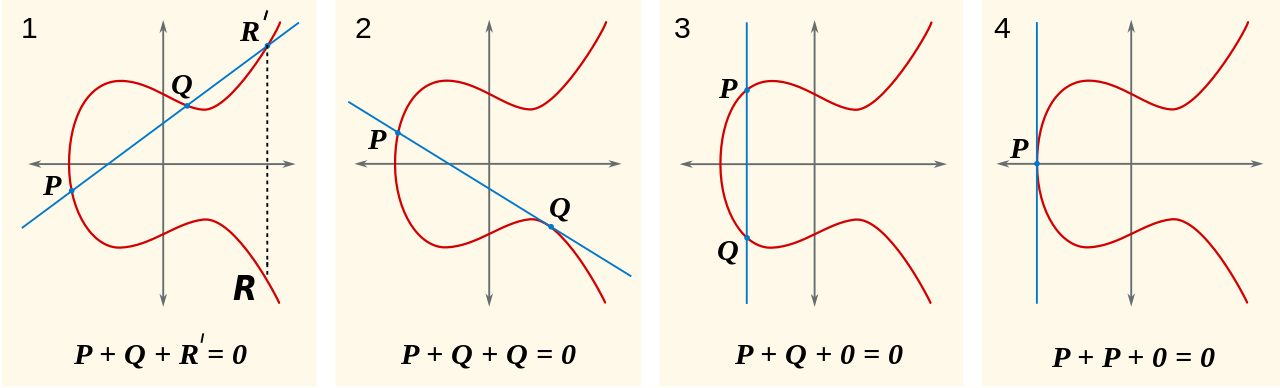
\includegraphics[scale=0.3]{images/ECClines.png} 
    \end{center}

    Заметим, что при таком задании операции '+' обратная точка в группе - это точка с противоположной координатой $y$. С помощью уравнений выразим операцию сложения в нормальных координатах: $A,B,C\in \E(\F_p),\q A=(x_1,y_1),\q B=(x_2,y_2), \q C=(x_3,y_3)$ и $A + B = C$, рассмотрим 3 случая: 
    \begin{enumerate}
      \item $x_1\neq x_2$. Обозначим $k := \frac{y_1-y_2}{x_1-x_2}$. Пусть $C:=A+B$ и $C=(x_3,y_3)$. Тогда
      \[x_3 = k^2 - x_1 - x_2\]
      \[y_3 = k(x_1 - x_3) - y_1\]
      \item $x_1 = x_2,\q y_1 = -y_2$. Тогда $A+B = \infty$.
      \item $A = B$. Обозначим $k := \frac{3x_1^2 + a}{2y_1}$. Тогда
      \[x_3 = k^2 - 2x_1\]
      \[y_3 = k(x_1 - x_3) - y_1\]
    \end{enumerate}

    Определим приватный метод twice для удвоения точки. Заметим, что если $y = 0$, то удвоение точки даст ноль:
    \begin{cppcode}
void twice() {
    if (m_is_null) {
        return;
    }

    if (!m_y.is_invertible()) {
        m_is_null = true;
        return;
    }

    const Element k = (m_field->element(3) * Element::pow(m_x, 2) + *m_a) / (m_y << 1);
    const Element x = Element::pow(k, 2) - (m_x << 1);
    m_y = k * (m_x - x) - m_y;
    m_x = x;
}
    \end{cppcode}
    Значит сложение точки будет:
    \begin{cppcode}
EllipticCurvePoint& operator+=(const EllipticCurvePoint& other) {
    if (m_is_null) {
        return *this = other;
    } else if (other.m_is_null) {
        return *this;
    }

    if (m_x == other.m_x) {
        if (m_y != other.m_y) {
            m_is_null = true;
        } else {
            twice();
        }

        return *this;
    }

    const Element k = (other.m_y - m_y) / (other.m_x - m_x);
    const Element x = Element::pow(k, 2) - m_x - other.m_x;
    m_y = k * (m_x - x) - m_y;
    m_x = x;

    return *this;
}
    \end{cppcode}
    \item Вычитать. Так как мы поняли, что
    \begin{cppcode}
void negative() {
    m_y = -m_y;
}
    \end{cppcode}
    то отрицанием и вычитанием будут:
    \begin{cppcode}
EllipticCurvePoint operator-() const {
    EllipticCurvePoint result = *this;
    result.negative();
    return result;
}

EllipticCurvePoint& operator-=(const EllipticCurvePoint& other) {
    EllipticCurvePoint temp = other;
    temp.negative();
    return *this += temp;
}

EllipticCurvePoint& operator-=(EllipticCurvePoint&& other) {
    other.negative();
    return *this += other;
}
    \end{cppcode}
    \item Умножаться на натуральное число.

    Умножение на число n - это сложение n раз точки с собой. Есть несколько этапов:
    \begin{enumerate}
      \item Представить число n в \textit{non-adjancent form}(NAF) форме - это уникальное представление числа в двоичном основании, где есть цифра $-1$. Такое представление помогает достичть минимального веса Хэмминга (количество цифр, отличных от 0), что заметно ускорит умножение точки на число, если удвоение точки будет быстрее сложения. Алгоритм перевода из двоичной системы исчисления в NAF: 

       \begin{algorithm}[H]
        \caption{NAF from binary}
        \KwData{$n=(n_{m-1}n_{m-2}\dots n_0)_2$}
        \KwResult{$z = (z_{m}z_{m-1}\dots z_1z_0)_{NAF}$}
        $i\gets 0$

        \While{$n > 0$} {
          \eIf{$n$ \rm is odd } {
            $z_i\gets 2 - (n\mod 4)$
            $n\gets n - z_i$
          } {
            $z_i\gets 0$
          }
          $n\gets n/2$

          $i\gets i+1$
        }
      \end{algorithm}
       Есть версия данного алгоритма, которая основана на битовых операциях:

      \begin{algorithm}[H]
        \caption{NAF from binary by bit operations}
        \KwData{$x=(x_{m-1}x_{m-2}\dots n_0)_2$}
        \KwResult{$z = (z_{m}z_{m-1}\dots z_1z_0)_{NAF}$}
        $xh\gets x >> 1$

        $x3\gets x + xh$

        $c\gets xh \text{ XOR } x3$

        $pb\gets x3 \text{ AND } c$

        $nb\gets xh \text{ AND } c$

        $z\gets pb - nb$
      \end{algorithm}
      Есть улучшенная версия данного представления:

      \begin{definition}
        Пусть $w\geqslant 2$ - положительное целое число. Тогда wNAF представление положительного числа $k$ - это представление $k=\sum_{i=0}^{l-1}k_i2^i$, где каждый ненулевой коэффициент $k_i$ нечётный, $|k_i|<2^{w-1}$, $k_{l-1}\neq 0$ и хотя бы одна ненулевая цифра есть в каждой подпоследовательности из $w$ цифр. Длина такого представления равна $l$. 
      \end{definition}
      \begin{theorem}[Свойства wNAF] Пусть $k$ - положительное целое число, тогда 
        \begin{enumerate}
          \item $k$ имеет уникальное представление wNAF, которое обозначается $NAF_w(k)$
          \item $NAF_2(k)=NAF(k)$, где $NAF(k)$ - это классическое бинарное представление в NAF 
          \item Длина $NAF_w(k)$ больше длины $(k)_2$ хотя бы на 1 цифру. 
          \item Средняя плотность ненулевых цифр в $wNAF$ представлении длины $l$ примерно $\frac{1}{w+1}$. 
        \end{enumerate}
      \end{theorem}
      Алгоритм вычисления $wNAF$ формы:

        \begin{algorithm}[H]
        \caption{Computing wNAF}
        \KwData{$w,k\in\N$}
          \KwResult{$NAF_w(k)$}
       $i\gets 0$

          \While{$k\geqslant 1$} {
            \eIf{$k$ is odd } {
              $k_i\gets k$ (mod $2^w$)
              $k\gets k - k_i$
            } {
              $k_i\gets 0$
            }
            $k_i\gets k/2$

            $i\gets i+1$
          }
          \Return $(k_{i-1},\dots,k_1,k_0)$
      \end{algorithm}
      \item Теперь напишем алгоритм вычисления кратной точки:

        \begin{algorithm}[H]
        \caption{wNAF for computing kP}
        \KwData{$w,k\in\N,P\in\E(\F_p)$}
          \KwResult{$Q:=kP$}
          $[k_i]\gets NAF_w(k)$

          Compute $P_i:=iP$ for $i\in \left\{1,3,5,\dots,2^{w-1}-1\right\}$

          $Q\gets \mathcal{O}$

          \For{$i$ from $l-1$ to 0} {
            $Q\gets 2Q$

            \If{$k_i\neq 0$} {
              \eIf{$k_i>0$} {
                $Q\gets Q + P_{k_i}$
              } {
                $Q\gets Q - P_{-{k_i}}$
              }
            }
          }
          \Return $Q$
      \end{algorithm}
    \end{enumerate}
    Имплементируем NAF как шаблон и подружим его с классом точки для быстрого зануления и удвоения:
    \begin{cppcode}
constexpr size_t c_width = 3;

struct Coefficient {
    uint16_t value;
    bool is_negative;
};

using WnafForm = std::vector<Coefficient>;

constexpr uint16_t c_mask_modulo_2_pow_w = (1 << c_width) - 1;

WnafForm get_wnaf(uint value) {
    WnafForm result;

    while (value > 0) {
        if ((value & 0b1) == 1) {
            uint16_t coef_value = value.convert_to<uint16_t>() & c_mask_modulo_2_pow_w;

            if (coef_value >= (1 << (c_width - 1))) {
                coef_value = (1 << c_width) - coef_value;
                result.push_back({.value = coef_value, .is_negative = true});
                value += coef_value;
            } else {
                result.push_back({.value = coef_value, .is_negative = false});
                value -= coef_value;
            }
        } else {
            result.push_back({.value = 0, .is_negative = false});
        }

        value >>= 1;
    }

    return result;
}

constexpr size_t c_k_number = static_cast<size_t>(1) << (c_width - 2);

template<typename T>
T wnaf_addition(T value, const uint& n) {
    WnafForm wnaf_form = get_wnaf(n);
    T two_value = value + value;
    std::vector<T> k_values = {value};

    for (size_t i = 1; i < c_k_number; ++i) {
        k_values.emplace_back(k_values.back() + two_value);
    }

    value.nullify();

    for (size_t i = wnaf_form.size(); i > 0; --i) {
        value.twice();

        if (wnaf_form[i - 1].value != 0) {
            if (!wnaf_form[i - 1].is_negative) {
                value += k_values[wnaf_form[i - 1].value >> 1];
            } else {
                value -= k_values[wnaf_form[i - 1].value >> 1];
            }
        }
    }

    return value;
}
    \end{cppcode}
    где
    \begin{cppcode}
void nullify() {
    m_is_null = true;
}
    \end{cppcode}
    Тогда умножение точки на число будет:
    \begin{cppcode}
EllipticCurvePoint& operator*=(const uint& value) {
    *this = wnaf_addition<EllipticCurvePoint>(*this, value);
    return *this;
}

EllipticCurvePoint& operator*=(const Element& element) {
    *this = wnaf_addition<EllipticCurvePoint>(*this, element.value());
    return *this;
}
    \end{cppcode}
    \item Сравнивать. Точки равны, если они обе нули или если у них совпадают координаты:
    \begin{cppcode}
friend bool operator==(const EllipticCurvePoint& lhs, const EllipticCurvePoint& rhs) {
    return (lhs.m_is_null && rhs.m_is_null) || (lhs.m_x == rhs.m_x && lhs.m_y == rhs.m_y);
}
    \end{cppcode}
    \item Приватный статический метод создания нулевой точки. За нулевую точку принято считать точку с координатами (0,1):
    \begin{cppcode}
static EllipticCurvePoint null_point(const std::shared_ptr<const Element>& a,
const std::shared_ptr<const Element>& b, const std::shared_ptr<const Field>& F) {
          return EllipticCurvePoint(F->element(0), F->element(1), a, b, F, true);
}    
    \end{cppcode}
    \item Стандартным образом определяем по 4 дружественных оператора на каждую операцию $+,-,*$ через их $+=$ версии.
    \item Делаем геттеры на x,y.
\end{itemize}
\subsection{Эллиптическая кривая}
По сути мы повторяем функционал класса поля:
\begin{cppcode}
class EllipticCurve {
    using Field = field::Field;
    using Element = field::FieldElement;

public:
    EllipticCurve(const Element& a, const Element& b, Field F);
    EllipticCurve(Element&& a, const Element& b, Field F);
    EllipticCurve(const Element& a, Element&& b, Field F);
    EllipticCurve(Element&& a, Element&& b, Field F);

    const Field& get_field() const;
    const Element& get_a() const;
    const Element& get_b() const;

private:
    std::shared_ptr<const Element> m_a;
    std::shared_ptr<const Element> m_b;
    std::shared_ptr<const Field> m_field;
};
\end{cppcode}
Этот класс должен поддерживать 3 вида создания точек:
\begin{itemize}
  \item Создание нулевой точки:
  \begin{cppcode}
EllipticCurvePoint null_point() const {
    return EllipticCurvePoint::null_point(m_a, m_b, m_field);
}
  \end{cppcode}
  \item Создание точки от x координаты. Но на эллиптической кривой может и не лежать данная координата, поэтому надо проверить, существует ли корень от $x^3 + ax + b$ в $\F_p$. Есть два варианта:
  \begin{enumerate}
    \item $p\equiv 3\mod 4$
    \item $p\equiv 1\mod 4$
  \end{enumerate}
  Почти все простые числа от NIST обладают первым свойством, поэтому рассмотрим только его. Но в реализации имплементирован и протестирован и второй случай.
  \begin{enumerate}
    \item Если число $a$ имеет корень $x\in\F_p\colon x^2 = a$, то $a$ либо равен 0, тогда корень понятно 0, либо лежит в $2\Z_{p - 1}$, так как $\F_p^*\cong \Z_{p-1}$.

  Пусть $p - 1=: 2k$. Значит $k = \frac{p-1}{2}$. Заметим, что тогда 
  \[\forall y \in 2\Z_{p - 1}\q \frac{p-1}{2}y = 0\] 
  Отсюда вытекает критерий: $\exists x\in\F_p\colon x^2 = a \Leftrightarrow a^{\frac{p-1}{2}} = 1$.
    \item Пусть $a^{\frac{p-1}{2}} = 1$. Так как $p\equiv 3\mod 4$, то $\frac{p-1}{2}$ нечётно, т.е.
    \[\frac{p-1}{2} = 2k - 1\implies \frac{p+1}{2} = 2k\]
    Тогда получаем, что
    \[a^{\frac{p-1}{2}} = 1\implies a^{\frac{p-1}{2}}\cdot a = a\]
    \[a = a^{\frac{p+1}{2}} = a^{2k}=(a^k)^2\]
    Значит в качестве корня подойдёт $x:= a^k = a^{\frac{p+1}{4}}$.

    Итого:
    \begin{cppcode}
std::optional<FieldElement> find_root(const FieldElement& value, const Field& field) {
    if (!value.is_invertible()) {
        return std::nullopt;
    }

    const uint& p = field.modulus();
    const FieldElement one = field.element(1);

    if (FieldElement::pow(value, (p - 1) >> 1) != one) {
        return std::nullopt;
    }

    return FieldElement::pow(value, (p + 1) >> 2);
}
    \end{cppcode}
    Используем std::optional для передачи того, можно ли найти корень или нет. Тогда методами эллиптической кривой будут:
    \begin{cppcode}
private:
std::optional<EllipticCurve::Element> EllipticCurve::find_y(const Element& x) const {
    Element value = Element::pow(x, 3) + *m_a * x + *m_b;
    return find_root(value, *m_field);
}

public:
std::optional<EllipticCurvePoint> point_with_x_equal_to(const Element& x) const {
    if (!x.is_invertible()) {
        return null_point();
    }

    std::optional<Element> y = find_y(x);

    if (!y.has_value()) {
        return std::nullopt;
    }

    return EllipticCurvePoint(x, std::move(y.value()), m_a, m_b, m_field);
}

std::optional<EllipticCurvePoint> point_with_x_equal_to(Element&& x) const {
    if (!x.is_invertible()) {
        return null_point();
    }

    std::optional<Element> y = find_y(x);

    if (!y.has_value()) {
        return std::nullopt;
    }

    return EllipticCurvePoint(std::move(x), std::move(y.value()), m_a, m_b, m_field);
}
    \end{cppcode}
    \item Создание точки по двум координатам. Надо проверить только, что координаты удовлетворяют уравнению кривой:
    \begin{cppcode}
private:
bool EllipticCurve::is_valid_coordinates(const Element& x, const Element& y) const {
    const Element lhs = Element::pow(y, 2);
    const Element rhs = Element::pow(x, 3) + *m_a * x + *m_b;
    return lhs == rhs;
}

bool EllipticCurve::is_null_coordinates(const Element& x, const Element& y) const {
    return x.value() == 0 && y.value() == 1;
}

public:
std::optional<EllipticCurvePoint> point(const Element& x, const Element& y) const {
    if (is_null_coordinates(x, y)) {
        return null_point();
    }

    if (!is_valid_coordinates(x, y)) {
        return std::nullopt;
    }

    return EllipticCurvePoint(x, y, m_a, m_b, m_field);
}

std::optional<EllipticCurvePoint> point(Element&& x, const Element& y) const {
    if (is_null_coordinates(x, y)) {
        return null_point();
    }

    if (!is_valid_coordinates(x, y)) {
        return std::nullopt;
    }

    return EllipticCurvePoint(std::move(x), y, m_a, m_b, m_field);
}

std::optional<EllipticCurvePoint> point(const Element& x, Element&& y) const {
    if (is_null_coordinates(x, y)) {
        return null_point();
    }

    if (!is_valid_coordinates(x, y)) {
        return std::nullopt;
    }

    return EllipticCurvePoint(x, std::move(y), m_a, m_b, m_field);
}

std::optional<EllipticCurvePoint> point(Element&& x, Element&& y) const {
    if (is_null_coordinates(x, y)) {
        return null_point();
    }

    if (!is_valid_coordinates(x, y)) {
        return std::nullopt;
    }

    return EllipticCurvePoint(std::move(x), std::move(y), m_a, m_b, m_field);
}
    \end{cppcode}
  \end{enumerate}
\end{itemize}


\ProvidesFile{elgamal.tex}

Теперь, когда мы определили все нужные методы, можем имплементировать алгоритмы шифрования на эллиптических кривых. Главные алгоритмы, которые мы рассмотрим: Эль-Гамаль и ECDSA. Остальные алгоритмы используют реализованные объекты аналогично тому, как мы будем использовать их в предстоящих алгоритмах.

\section{Эллиптический Эль-Гамаль}
Общие данные: простое число $p$, эллиптическая кривая $\E(\F_p)$, точка на этой кривой $P\in\E(\F_p)$, её порядок $q$, отображение сообщения на эллиптическую кривую и обратное слева к нему отображение.

  Допустим Боб хочет отправить сообщение $m$ Алисе. Тогда:
  \begin{enumerate}
    \item Алиса генерирует секретный ключ $n_\alpha\colon 1\leqslant n_\alpha<q$, публичный ключ: $A:=n_\alpha P$. Отправляет публичный ключ Бобу.
    \item Боб обратимо отображает сообщение $m$ на эллиптическую кривую: $M\in\E(\F_p)$, генерирует одноразовый сектретный ключ $k\colon 1\leqslant k<q$, вычисляет $C_1:=kP,\q C_2:=kA+M$ и отправляет пару $(C_1,C_2)$ Алисе.
    \item Алиса вычисляет исходную точку по формуле:
    \[C_2 - n_\alpha C_1 =\]\[= kA+M - n_\alpha k P = n_\alpha k P + M - n_\alpha k P = M\]
    и отображает её обратно в $m$ 
  \end{enumerate}
  
  Отображать сообщение, представленное в виде двоичного числа, на эллиптическую кривую можно следующим образом:
  \begin{enumerate}
    \item Пусть наше поле $\F_p$, и $p$ - это достаточно большое число. Обозначим за $q$ - длину числа $p$ в битовом представлении.
    \item Выберем и зафиксируем число $l\in (0, \frac{q}{2})$, и будем в первые $l$ бит числа записывать наше сообщение $m$ в двоичном представлении.
    \item Заполним оставшиеся биты случайно. Тогда высока вероятность, что полученное число - это координата $x$ какой-то точки на эллиптической кривой. Если нет, то повторяем этот шаг, пока не получим точку на кривой.
    \item Когда Алиса посчитала точку $M$, она берёт координату $x$ этой точки. Тогда первые $l$ бит значения этой координаты и будут сообщением $m$. 
  \end{enumerate}

  Заметим, что отображать сообщения на кривую и обратно не является удобным. В вариации Эль-Гамаля с хешированием, выбирается хеш-функция $H\colon \E(\F_p)\to \left\{0,1\right\}^n$ и $(C_1,c_2) := (kP, m \oplus H(kA))$, т.е. сообщение в двоичном виде длины $\leqslant n$ XORится с хешем от точки $kA$. Тогда Алиса получает исходное сообщение через $m = c_2 \oplus H(n_\alpha C_1)$.

Реализуем данный функционал через класс:
\subsection{Каркас}
Запрашиваем нужные общие данные:
\begin{cppcode}
class ElGamal {
    using Curve = EllipticCurve;
    using Point = EllipticCurvePoint;

public:
    ElGamal(const Curve& curve, const Point& generator, const uint& generator_order);

private:

    Curve m_curve;
    Point m_generator;
    uint m_generator_order;
};
\end{cppcode}
\subsection{Методы}
Нам нужны методы
\begin{enumerate}
  \item Генерации ключей.

  Для этого нужнен генератор рандомных чисел. Обычный мерсен не подойдёт, так как он не предназначен для криптографии. Используем \href{https://github.com/Duthomhas/CSPRNG}{библиотеку CSPRNG} для этих целей. Она использует внутренние генераторы операционной системы. Напишем генератор рандомных uint:
  \begin{cppcode}
#include "csprng/csprng.hpp"

constexpr size_t c_size = 512 / sizeof(uint32_t);

uint generate_random_uint() {
    duthomhas::csprng rng;
    std::seed_seq sseq {228};
    rng.seed(sseq);
    uint result = 0;
    uint32_t x = rng(uint32_t());
    std::vector<uint32_t> values = rng(std::vector<uint32_t>(c_size));

    for (size_t i = 0; i < c_size; ++i) {
        result <<= 32;
        result += values[i];
    }

    return result;
}

uint generate_random_uint_modulo(const uint& modulus) {
    return generate_random_uint() % modulus;
}

uint generate_random_non_zero_uint_modulo(const uint& modulus) {
    return generate_random_uint_modulo(modulus - 1) + 1;
}
  \end{cppcode}

  Тогда ключи получаем через:
  \begin{cppcode}
struct Keys {
    uint private_key;
    Point public_key;
};

Keys ElGamal::generate_keys() const {
    uint private_key = generate_random_non_zero_uint_modulo(m_generator_order);
    Point public_key = private_key * m_generator;
    return Keys {.private_key = private_key, .public_key = public_key};
}
  \end{cppcode}
  \item Шифрование сообщения. Есть два варианта - нам предоставили уже готовое сообщение $M\in\E(\F_p)$, либо надо самим отобразить $m$ на кривую. Напишем отображение uint на кривую, через вероятностный алгоритм:
  \begin{cppcode}
size_t actual_bit_size(uint value) {
    size_t result = 0;

    while (value != 0) {
        ++result;
        value >>= 1;
    }

    return result;
}

static std::map<uint, uint> p_zero_mask;
static constexpr uint c_full_bits = uint(0) - 1;

ElGamal::Point ElGamal::map_to_curve(const uint& message) const {
    const Field& F = m_curve.get_field();
    const uint& p = F.modulus();

    if (!p_zero_mask.contains(p)) {
        const size_t l = actual_bit_size(p) >> 1;
        uint zero_mask = (c_full_bits >> l) << l;
        p_zero_mask.insert({p, zero_mask});
    }

    const uint& zero_mask = p_zero_mask.at(p);

    for (;;) {
        uint x = random::generate_random_uint_modulo(p);
        x &= zero_mask;
        x |= message ^ (message & zero_mask);
        auto opt = m_curve.point_with_x_equal_to(F.element(x));

        if (opt.has_value()) {
            return opt.value();
        }
    }
}
  \end{cppcode}
  Так как нам нужно быстро записывать сообщение в половину длины простого числа, то нам нужна нулевая маска для этой половины. Заводим статическую мапу, которая будет хранить предподсчитанные маски, и создаём новые маски, если такого простого числа p не встречалось за время выполнения.

  Отображение обратно с точки на uint происходит аналогично:
  \begin{cppcode}
uint ElGamal::map_to_uint(const Point& message) const {
    const uint& p = m_curve.get_field().modulus();

    if (!p_zero_mask.contains(p)) {
        const size_t l = actual_bit_size(p) >> 1;
        uint zero_mask = (c_full_bits >> l) << l;
        p_zero_mask.insert({p, zero_mask});
    }

    const uint& zero_mask = p_zero_mask.at(p);
    uint x = message.get_x().value();
    x ^= (x & zero_mask);
    return x;
}
  \end{cppcode}
  Заметим, что мы обрезаем сообщение, если количество бит в нём больше, чем половина бит от простого модуля. С высокой долей вероятности, этот алгоритм будет работать относительно быстро и при большей заполненности бит простого модуля, поэтому вы можете поэксперементировать над длиной нулевой маски.

  Имея оба отображения, можем имплементировать алгоритм шифрования, описанный ранее:
  \begin{cppcode}
struct EncryptedMessage {
    Point generator_degree;
    Point message_with_salt;
};

EncryptedMessage encrypt(const Point& message, const Point& public_key) const {
    const uint k = generate_random_non_zero_uint_modulo(m_generator_order);
    const Point generator_degree = k * m_generator;
    const Point message_with_salt = message + k * public_key;
    return {.generator_degree = generator_degree, .message_with_salt = message_with_salt};
}

EncryptedMessage encrypt(const uint& message, const Point& public_key) const {
    Point point_message = map_to_curve(message);
    return encrypt(point_message, public_key);
}
  \end{cppcode}
  \item Дешифрование. По алгоритму, описанному ранее:
  \begin{cppcode}
Point decrypt_to_point(const EncryptedMessage& encrypted_message, const uint& private_key) const {
    return encrypted_message.message_with_salt - private_key * encrypted_message.generator_degree;
}

uint decrypt_to_uint(const EncryptedMessage& encrypted_message, const uint& private_key) const {
    const Point M = encrypted_message.message_with_salt
                    - private_key * encrypted_message.generator_degree;
    return map_to_uint(M);
}

  \end{cppcode}
\end{enumerate}

Итого сигнатура класса:
\begin{cppcode}
class ElGamal {
    using Curve = EllipticCurve;
    using Point = EllipticCurvePoint;

public:
    struct Keys {
        uint private_key;
        Point public_key;
    };

    struct EncryptedMessage {
        Point generator_degree;
        Point message_with_salt;
    };

    ElGamal(const Curve& curve, const Point& generator, const uint& generator_order);

    Keys generate_keys() const;

    EncryptedMessage encrypt(const uint& message, const Point& public_key) const;
    EncryptedMessage encrypt(const Point& message, const Point& public_key) const;
    Point decrypt_to_point(const EncryptedMessage& encrypted_message, const uint& private_key) const;
    uint decrypt_to_uint(const EncryptedMessage& encrypted_message, const uint& private_key) const;

private:
    Point map_to_curve(const uint& message) const;
    uint map_to_uint(const Point& message) const;

    Curve m_curve;
    Point m_generator;
    uint m_generator_order;
};
\end{cppcode}


\ProvidesFile{ecdsa.tex}

\section{ECDSA}
Реализация вдохновлена \cite{das2004guideprotocols}

У этого алгоритма есть несколько основных подалгоритмов:
    \begin{enumerate}
      \item Алгоритм генерации основных параметров: 

      Пользователь выбирает простое число $p$ и уровень безопасности $L\colon 160\leqslant L\leqslant [\log_2 p]$ и $2^L\geqslant 4 \sqrt{p}$. На выходе получаем основные параметры эллиптической кривой.

      \begin{enumerate}
        \item Выбираем верифицировано случайным образом $a,b\in \F_p\colon 4a^3+27b^2\neq 0$, чтобы они были параметрами эллиптической кривой. Назовём её $\E(\F_p)$
        \item Находим $N:=\#\E(\F_p)$
        \item Проверяем, что существует простое число $n\geqslant 2^L\colon N \equiv 0$ (mod $n$), т.е. что у $N$ в делителях есть большое простое число. Если это условие неверно, то переходим на первый шаг
        \item Проверяем, что для этого простого числа $p^k-1\not\equiv 0$ (mod $n$) $\forall k\in \left\{1,2,\dots,20\right\}$
        \item Проверим, что $p\neq n$, иначе переходим на шаг 1
        \item Пусть $h:=\frac{N}{n}$
        \item Генерируем случайную точку $G'\in \E(\F_p)$ и задаём $G:=hG'$. Если $G=\mathcal{O}$, то повторяем данный шаг.
        \item Возвращаем $D:=(p, a, b, F, E, G, n, h)$
      \end{enumerate}
      \item Алгоритм генерации ключей:

      Пользователь передаёт основные параметры $D$. На выходе получаем открытый и закрытый ключи.

      \begin{enumerate}
        \item Выбираем случайное число $d\in \left\{1,\dots,n-1\right\}$
        \item Вычисляем $Q:=dG$
        \item Возвращаем $(Q,d)$, где точка на эллиптической кривой $Q$ - открытый ключ, а $d\in\N$ - закрытый ключ
      \end{enumerate}

      \item Алгоритм генерации цифровой подписи:

      Пользователь, который имеет основные параметры $D$ и ключи $(Q,d)$, хочет подписать сообщение $m$. Пусть $H$ - криптографическая хеш-функция, результат которой даёт число, битовое представление которого имеет длину не более $n$. На выходе получаем подпись $(r,s)$:

      \begin{enumerate}
        \item Выбираем случайное число $k\in \left\{1,\dots,n-1\right\}$
        \item Вычисляем точку $(x_1,y_1)= kG$
        \item Вычисляем $r := x_1$ (mod $n$). Если $r=0$, то переходим к шагу 1
        \item Вычисляем $e := H(m)$
        \item Вычисляем $s := k^{-1}(e+dr)$ (mod $n$). Если $s=0$, то переходим к шагу 1
        \item Возвращаем $(r,s)$
      \end{enumerate}

      \item Алгоритм проверки цифровой подписи:

      Другой пользователь получает основные параметры $D$, хеш-функцию $H$, сообщение $m$, подпись $(r,s)$ и открытый ключ $Q$ от первого пользователя и хочет проверить подпись. На выходе получаем решение о принятии или отклонении подписи:

      \begin{enumerate}
        \item Если $r,s$ - это не целые числа, принадлежащие $[1,n-1]$, то отклоняем
        \item Вычисляем $e:=H(m)$
        \item Вычисляем $w := s^{-1} = k(e+dr)^{-1}$ (mod $n$) 
        \item Вычисляем $u_1:=ew$ (mod $n$) и $u_2:=rw$ (mod $n$)
        \item Вычисляем координаты точки $X=(x_1,y_1):=u_1G+u_2Q$
        \item Если $X=\mathcal{O}$, то отклоняем
        \item Вычисляем $v:=x_1$ (mod $n$)
        \item Если $v = r$, то принимаем, иначе отклоняем
      \end{enumerate}
    \end{enumerate}

Алгоритм генерации основных параметров не нужен при использовании кривых от NIST, но всё же имплементирован в реализации. Рассмотрим ECDSA без генерации основных параметров:
\subsection{Каркас}
Аналогично Эль-Гамалю, мы хотим общие данные, т.е. основные параметры:
\begin{cppcode}
class ECDSA {
    using Element = FieldElement;
    using Curve = EllipticCurve;
    using Point = EllipticCurvePoint;

public:
    ECDSA(const Curve& elliptic_curve, const Point& generator, const uint& n, const uint& h);

private:
    Curve m_elliptic_curve;
    Point m_generator;
    uint m_n;
    uint m_h;
};
  \end{cppcode}
\subsection{Методы}
Так как это алгоритм для генерации и проверки цифровой подписи, то у него всего 3 метода:
\begin{itemize}
  \item Генерация ключей: аналогична Эль-Гамалю:
  \begin{cppcode}
struct Keys {
    Point public_key;
    uint private_key;
};

Keys ECDSA::generate_keys() const {
    uint d = generate_random_non_zero_uint_modulo(m_n);
    Point Q = d * m_generator;
    return {.public_key = Q, .private_key = d};
}
  \end{cppcode}
  \item Генерация цифровой подписи: это вероятностный алгоритм, поэтому используем конструкцию for(;;) для удобных прыжков:
  \begin{cppcode}
struct Signature {
    uint r;
    uint s;
};

ECDSA::Signature ECDSA::generate_signature(const uint& private_key, const uint& message) const {
    const Field F(m_n);

    for (;;) {
        const Element k = random::generate_random_non_zero_field_element(F);

        const Point P = k * m_generator;
        const uint& r = P.get_x().value();

        if (r == 0) {
            continue;
        }

        const Element edr = F.element(message) + F.element(private_key) * F.element(r);
        const uint& s = (Element::inverse(k) * edr).value();

        if (s == 0) {
            continue;
        }

        return {.r = r, .s = s};
    }

    return {};
}
  \end{cppcode}
  \item Проверка цифровой подписи: ничего нового, просто следуем алгоритму:
  \begin{cppcode}
bool ECDSA::is_correct_signature(const Point& public_key, const uint& message,
                                 const Signature& signature) const {
    const uint& r = signature.r;
    const uint& s = signature.s;

    if (r == 0 || s == 0) {
        return false;
    }

    if (r >= m_n || s >= m_n) {
        return false;
    }

    const Field F = Field(m_n);
    const Element w = Element::inverse(F.element(s));
    const Element u1 = F.element(message) * w;
    const Element u2 = F.element(r) * w;
    const Point X = u1 * m_generator + u2 * public_key;

    if (X.is_zero()) {
        return false;
    }

    const uint& v = X.get_x().value();
    return v == r;
}
  \end{cppcode}
\end{itemize}

Итого сигнатура класса:
\begin{cppcode}
class ECDSA {
    using Field = field::Field;
    using Element = field::FieldElement;
    using Curve = elliptic_curve::EllipticCurve;
    using Point = elliptic_curve::EllipticCurvePoint<elliptic_curve::CoordinatesType::Normal>;

public:
    struct Keys {
        Point public_key;
        uint private_key;
    };

    struct Signature {
        uint r;
        uint s;
    };

    ECDSA(const Field& field, const Curve& elliptic_curve, const Point& generator, const uint& n,
          const uint& h);

    Keys generate_keys() const;
    Signature generate_signature(const uint& private_key, const uint& message) const;
    bool is_correct_signature(const Point& public_key, const uint& message,
                              const Signature& signature) const;

private:
    Field m_field;
    Curve m_elliptic_curve;
    Point m_generator;
    uint m_n;
    uint m_h;
};
\end{cppcode}


\ProvidesFile{tests.tex}

\section{Тестирование}
Проведено тестирование на корректность и на устойчивость для всех реализованных в данном руководстве классов, поэтому все имплементированные классы являются корректными. Тесты, как и способы их запустить, находятся в этом же репозитории.

Отдельно хочется отметить скорость выполнения операций у самописного класса uint\_t относительно скорости длинки от буста. Вот результаты замеров времени работы при одинаковой нагрузке:
\begin{itemize}
  \item Debug сборка:

    TODO

  \item Release сборка:

    TODO
\end{itemize}

Мы сравнялись почти во всех операциях, кроме умножения и деления, которые занимают в два раза больше времени относительно бустовских. Это достаточно неплохой результат, поэтому можно продолжать дальнейшие оптимизации данного класса.

Результаты времени работы шифрования и цифровой подписи реализованных классов и готовых решений:
\begin{itemize}
  \item Debug сборка:

    TODO

  \item Release сборка:

    TODO
\end{itemize}

Вывод: TODO


\ProvidesFile{specialization.tex}

\section{Специализация}
Остановимся на конкретной кривой и генераторе, а именно \href{https://neuromancer.sk/std/nist/P-256}{NIST P-256}. Будем писать однофайловое решение шифрования эллиптическим Эль-Гамалем. Начнём!

\subsection{Поле}
Так как нам нужно одно конкретное поле, то можно соединить классы FieldElement и uint\_t в одно целое, забыв о классе Field:
\begin{cppcode}
class F_256 {
    static constexpr size_t c_bits = 512;
    static constexpr size_t c_bits_in_byte = 8;
    static constexpr size_t c_digit_size = 32;
    static constexpr size_t c_digit_number = 16;
    static constexpr size_t c_half_digit_number = 8;

    using digits = std::array<uint32_t, c_digit_number>;
    digits m_digits = {};
}
\end{cppcode}
\subsubsection{Арифметика}
Так как наше простое число имеет 256 бит, то достаточно 512 бит для сдерживания переполнения. Для нормализации числа нам нужно определить само простое число p, но вот загвоздка --- оно то тоже 256 битное, а мы не можем определить статическое поле класса самим классом. Поэтому идём на хитрость: расписываем через constexpr только цифры простого числа:
\begin{cppcode}
static constexpr digits p_values = {4294967295U, 4294967295U, 4294967295U, 0U, 0U, 0U, 1U, 4294967295U};
\end{cppcode}
Тогда для прибавления и вычитания простого числа при нормализации числа определим приватные методы, которые не проверяют инвариант:
\begin{cppcode}
constexpr void add_p_uncheck() {
    uint32_t carry = 0;

    for (size_t i = 0; i < c_digit_number; ++i) {
        uint32_t sum = carry + p_values[i];
        m_digits[i] += sum;
        carry = (m_digits[i] < sum) || (sum < carry);
    }
}

constexpr void subtract_p_uncheck() {
    uint32_t remainder = 0;

    for (size_t i = 0; i < c_digit_number; ++i) {
        uint32_t prev = m_digits[i];
        uint32_t sum = p_values[i] + remainder;
        m_digits[i] -= sum;
        remainder = (m_digits[i] > prev) || (sum < remainder);
    }
}
\end{cppcode}
Теперь модифицируем инкремент и декремент: так как мы считаем, что при инкременте число поддерживало инвариант, то максимум кем оно могло стать --- это самим простым модулем p, поэтому:
\begin{cppcode}
constexpr void increment() {
    for (size_t i = 0; i < c_digit_number; ++i) {
        m_digits[i] += 1;

        if (m_digits[i] != 0) {
            break;
        }
    }

    if (m_digits == p_values) {
        m_digits = {};
    }
}
\end{cppcode}
С декрементом немного посложней. Единственный особый переполнение --- это декремент от 0. Но мы знаем, чему число тогда станет равно: $p-1$, поэтому заранее определим его:
\begin{cppcode}
static constexpr digits max_mod_p = {4294967294U, 4294967295U, 4294967295U, 0U, 0U, 0U, 1U, 4294967295U};

constexpr void decrement() {
    if (*this == 0) {
        m_digits = max_mod_p;
        return;
    }

    for (size_t i = 0; i < c_digit_number; ++i) {
        uint32_t temp = m_digits[i];
        m_digits[i] -= 1;

        if (temp >= m_digits[i]) {
            break;
        }
    }
}
\end{cppcode}
Оператором отрицания будет как обычно вычитание из модуля или 0, если текущее значение 0:
\begin{cppcode}
constexpr F_256 operator-() const {
    if (!is_invertible()) {
        return *this;
    }

    digits result = p_values;
    uint32_t remainder = 0;

    for (size_t i = 0; i < c_digit_number; ++i) {
        uint32_t prev = result[i];
        uint32_t sum = m_digits[i] + remainder;
        result[i] -= sum;
        remainder = (result[i] > prev) || (sum < remainder);
    }

    return F_256(result);
}
\end{cppcode}
Теперь можно определить операции сложения и вычитания:
\begin{cppcode}
constexpr F_256& operator+=(const F_256& other) {
    uint32_t carry = 0;

    for (size_t i = 0; i < c_digit_number; ++i) {
        uint32_t sum = carry + other[i];
        m_digits[i] += sum;
        carry = (m_digits[i] < sum) || (sum < carry);
    }

    if (!is_valid()) {
        subtract_p_uncheck();
    }

    return *this;
}

constexpr F_256& operator-=(const F_256& other) {
    uint32_t remainder = 0;

    for (size_t i = 0; i < c_digit_number; ++i) {
        uint32_t prev = m_digits[i];
        uint32_t sum = other[i] + remainder;
        m_digits[i] -= sum;
        remainder = (m_digits[i] > prev) || (sum < remainder);
    }

    if (!is_valid()) {
        add_p_uncheck();
    }

    return *this;
}
\end{cppcode}
\subsubsection{Умножение}
Чтобы редуцировать число, которое получиться после умножения двух чисел из поля, нам надо научиться брать по модулю число $c\colon 0\leqslant c < p^2$. У P-256 есть специальный ритуал для этого:
\begin{cppcode}
constexpr void reduce() {
    F_256 s1({m_digits[0],
              m_digits[1],
              m_digits[2],
              m_digits[3],
              m_digits[4],
              m_digits[5],
              m_digits[6],
              m_digits[7]});
    F_256 s2({0, 0, 0, m_digits[11], m_digits[12], m_digits[13], m_digits[14], m_digits[15]});
    F_256 s3({0, 0, 0, m_digits[12], m_digits[13], m_digits[14], m_digits[15], 0});
    F_256 s4({m_digits[8], m_digits[9], m_digits[10], 0, 0, 0, m_digits[14], m_digits[15]});
    F_256 s5({m_digits[9],
              m_digits[10],
              m_digits[11],
              m_digits[13],
              m_digits[14],
              m_digits[15],
              m_digits[13],
              m_digits[8]});
    F_256 s6({m_digits[11], m_digits[12], m_digits[13], 0, 0, 0, m_digits[8], m_digits[10]});
    F_256 s7({m_digits[12], m_digits[13], m_digits[14], m_digits[15], 0, 0, m_digits[9], m_digits[11]});
    F_256 s8({m_digits[13],
              m_digits[14],
              m_digits[15],
              m_digits[8],
              m_digits[9],
              m_digits[10],
              0,
              m_digits[12]});
    F_256 s9({m_digits[14], m_digits[15], 0, m_digits[9], m_digits[10], m_digits[11], 0, m_digits[13]});
    *this = s1 + s2 + s2 + s3 + s3 + s4 + s5 - s6 - s7 - s8 - s9;
}
\end{cppcode}
Умные дяди написали, что нужно именно так, поэтому мы как макаки повторяем. Значит умножение мы крадём у uint\_t и в конце редуцируем:
\begin{cppcode}
friend constexpr F_256 operator*(const F_256& lhs, const F_256& rhs) {
    F_256 result;

    for (size_t i = 0; i < c_half_digit_number; ++i) {
        uint64_t u = 0;

        for (size_t j = 0; j < c_half_digit_number; ++j) {
            u = static_cast<uint64_t>(result[i + j])
              + static_cast<uint64_t>(lhs[i]) * static_cast<uint64_t>(rhs[j]) + (u >> c_digit_size);
            result[i + j] = static_cast<uint32_t>(u);
        }

        result[i + c_half_digit_number] = static_cast<uint32_t>(u >> c_digit_size);
    }

    result.reduce();
    return result;
}
\end{cppcode}
Заметим, что используется только половины длины числа, так как мы считаем, что lhs и rhs удовлетворяют инваринату: lhs, rhs < p, а количество цифр в $p$ --- это 8 = c\_half\_digit\_number.
\subsubsection{Инверсия}
Так как мы хотим всё и быстро, то у нас нет целочисленного деления. Но как же реализовать инверсию без деления? На помощь приходит алгоритм бинарного расширенного евклида. В его основе лежит житейская мудрость: не можешь использовать обычную арифметику --- используй бинарную. Так и поступил автор данного алгоритма. Пруфов работы не будет (точнее, объяснение есть в \cite{das2004guide}):
\begin{cppcode}
constexpr void inverse() {
    constexpr F_256 zero;
    constexpr F_256 one = 1;

    F_256 u = *this;
    F_256 v(p_values);

    F_256 x_1 = one;
    F_256 x_2;

    while (u != one && v != one) {
        while (u.is_even()) {
            u >>= 1;

            if (x_1.is_even()) {
                x_1 >>= 1;
            } else {
                x_1.add_p_uncheck();
                x_1 >>= 1;
                assert(x_1.is_valid());
            }
        }

        while (v.is_even()) {
            v >>= 1;

            if (x_2.is_even()) {
                x_2 >>= 1;
            } else {
                x_2.add_p_uncheck();
                x_2 >>= 1;
                assert(x_2.is_valid());
            }
        }

        if (u >= v) {
            u -= v;
            x_1 -= x_2;
        } else {
            v -= u;
            x_2 -= x_1;
        }
    }

    if (u == 1) {
        *this = x_1;
    } else {
        *this = x_2;
    }

    assert(is_valid());
}
\end{cppcode}
\subsubsection{Пролом 4 стены}
Нам нужен быстрый доступ к данным, поэтому открываем пользователю методы:
\begin{cppcode}
const uint32_t& first_digit() const {
    return m_digits[0];
}

constexpr const uint32_t& operator[](size_t pos) const {
    return m_digits[pos];
}

constexpr uint32_t& operator[](size_t pos) {
    return m_digits[pos];
}
\end{cppcode}
Да, это не безопасно, зато быстро.
\subsubsection{Конверсия}
У нас нет деления, значит мы можем привести только к 16,8,2-ичным системам счисления. Ограничимся для нашей специализации 16-ричной системой.

Основная сложность - каждая цифра содержит 8 16-ричных символов, поэтому нам понадобятся некоторые лямбды, которые будут упрощать деление числа на хекс-символы.

Так как мы начинаем заполнять со старших битов, то нам нужно пропустить верхние нули. Для цифр это несложно, но вот для скипа нулей внутри цифры нам придётся передать флаг в лямбды.

Итого:
\begin{cppcode}
constexpr std::string convert_to_hex_string() const {
    std::string result;
    size_t pos = c_digit_number;

    while (pos > 0 && m_digits[pos - 1] == 0) {
        --pos;
    }

    if (pos == 0) {
        return "0x0";
    }

    result += "0x";

    auto mini_push = [&](const uint8_t& value) {
        if (value < 10) {
            result.push_back(value + '0');
        } else {
            result.push_back(value - 10 + 'A');
        }
    };

    auto push = [&](const uint32_t& value, bool first_time = false) {
        size_t shift = 32;
        uint8_t temp = 0;

        if (first_time) {
            while (shift > 0 && temp == 0) {
                shift -= 4;
                temp = (value >> shift) & 0xF;
            }

            do {
                mini_push(temp);

                if (shift == 0) {
                    break;
                }

                shift -= 4;
                temp = (value >> shift) & 0xF;
            } while (shift >= 0);

            return;
        }

        while (shift > 0) {
            shift -= 4;
            temp = (value >> shift) & 0xF;
            mini_push(temp);
        }
    };

    push(m_digits[pos - 1], true);
    --pos;

    while (pos > 0) {
        push(m_digits[pos - 1]);
        --pos;
    }

    return result;
}
\end{cppcode}
Остальные методы без изменений.
\subsection{Точка Эллиптической кривой}
Забываем о классе эллиптической кривой и захардкоживаем внутрь класса точки основные параметры:
\begin{cppcode}
class EllipticCurvePoint {
    static constexpr F_256 c_a = "0xffffffff00000001000000000000000000000000fffffffffffffffffffffffc";
    static constexpr F_256 c_b = "0x5ac635d8aa3a93e7b3ebbd55769886bc651d06b0cc53b0f63bce3c3e27d2604b";
    static constexpr F_256 c_p_1 = "0x7FFFFFFF800000008000000000000000000000007FFFFFFFFFFFFFFFFFFFFFFF";
    static constexpr F_256 c_p_2 = "0x3FFFFFFFC0000000400000000000000000000000400000000000000000000000";

    F_256 m_x;
    F_256 m_y;
    bool m_is_null;
};
\end{cppcode}
где $p_1$ и $p_2$ - те самые значения, которые мы считали при нахождении корня в поле:
\[p_1:=\frac{p-1}{2}\]
\[p_2:=\frac{p+1}{4}\]
Они понадобятся нам для имплементации приватного метода нахождения y-координаты. Заметим, что $p\equiv 3\mod 4$, поэтому можно использовать прежний алгоритм:
\begin{cppcode}
static constexpr std::optional<F_256> find_y(const F_256& x) {
    F_256 value = F_256::pow(x, 3) + c_a * x + c_b;

    if (!value.is_invertible()) {
        return std::nullopt;
    }

    if (F_256::pow(value, c_p_1) != F_256(1)) {
        return std::nullopt;
    }

    return F_256::pow(value, c_p_2);
}
\end{cppcode}
В остальном никаких изменений методов нет, мы просто копируем используемые алгоритмы, например wNAF, в наш файл и подставляем в нужные места.
\subsection{Эль-Гамаль}
Так как нам больше не нужно держать общие данные, то класс Эль-Гамаль распадается на обычный namespace:
\begin{cppcode}
namespace ElGamal {
    using Point = EllipticCurvePoint;

    namespace {
        static constexpr Point m_generator =
            Point(F_256("0x6b17d1f2e12c4247f8bce6e563a440f277037d812deb33a0f4a13945d898c296"),
                  F_256("0x4fe342e2fe1a7f9b8ee7eb4a7c0f9e162bce33576b315ececbb6406837bf51f5"));
        static constexpr F_256 m_generator_order =
            "0xffffffff00000000ffffffffffffffffbce6faada7179e84f3b9cac2fc632551";

        Point map_to_curve(const F_256& message) {
            for (;;) {
                F_256 x = generate_random_non_zero_value_modulo(m_generator_order);

                for (size_t i = 0; i < 6; ++i) {
                    x[i] = message[i];
                }

                auto opt = Point::point_with_x_equal_to(x);

                if (opt.has_value()) {
                    return opt.value();
                }
            }
        }

        F_256 map_to_uint(const Point& message) {
            F_256 result;
            const F_256& x = message.get_x();

            for (size_t i = 0; i < 6; ++i) {
                result[i] = x[i];
            }

            return result;
        }
    }   // namespace

    struct Keys {
        F_256 private_key;
        Point public_key;
    };

    struct EncryptedMessage {
        Point generator_degree;
        Point message_with_salt;
    };

    constexpr Keys generate_keys() {
        F_256 private_key = generate_random_non_zero_value_modulo(m_generator_order);
        Point public_key = private_key * m_generator;
        return Keys {.private_key = private_key, .public_key = public_key};
    }

    EncryptedMessage encrypt(const F_256& message, const Point& public_key) {
        const F_256 k = generate_random_non_zero_value_modulo(m_generator_order);
        const Point generator_degree = k * m_generator;
        const Point message_with_salt = map_to_curve(message) + k * public_key;
        return {.generator_degree = generator_degree, .message_with_salt = message_with_salt};
    }

    F_256 decrypt(const EncryptedMessage& encrypted_message, const F_256& private_key) {
        Point M = encrypted_message.message_with_salt - private_key * encrypted_message.generator_degree;
        return map_to_uint(M);
    }
};   // namespace ElGamal
\end{cppcode}
Имплементация функций остаётся прежней, кроме того факта, что мы используем 6 бит из 8, вместо 4 бит, во время отображения сообщения на кривую и обратно. Это позволяет значительно увеличить передаваемое сообщение.
\subsection{Тестирование}
Наконец мы можем побаловаться с шифрованием сообщений через консоль:
\begin{cppcode}
int main() {
    std::cout << "Enter hexadecimal message:\n";
    std::string msg;
    std::cin >> msg;
    F_256 message = msg.c_str();
    std::cout << "Generating keys...\n";
    auto keys = ElGamal::generate_keys();
    std::cout << "Encrypting message...\n";
    auto encrypted_message = ElGamal::encrypt(message, keys.public_key);
    std::cout << "Decrypting message...\n";
    auto decrypted_message = ElGamal::decrypt(encrypted_message, keys.private_key);
    std::cout << "Decrypted message is:\n";
    std::string decrypted_msg = decrypted_message.convert_to_hex_string();
    std::cout << decrypted_msg << '\n';
    std::cout << "Checking correctness...\n";

    if (message != decrypted_message) {
        std::cout << "Fail ";

        if (msg.ends_with(decrypted_msg.substr(2))) {
            std::cout << "due to insufficient number of encryption bits\n";
        } else {
            std::cout << "due to implementation problems\n";
        }
    } else {
        std::cout << "Success!\n";
    }
}
\end{cppcode}
Результаты замеров тестов, сравнивая с шаблонным многофайловым решением:
\begin{itemize}
  \item Debug сборка:

    TODO

  \item Release сборка:

    TODO
\end{itemize}

Вывод: TODO


\ProvidesFile{conclusion.tex}

\section{Заключение}
За время этого гайда вы ознакомились с основными проблемами при попытке реализации криптографии на эллиптических кривых и узнали способы их решения. Это руководство является всего лишь вершиной айсберга такого вида криптографии, но я надеюсь, что оно поможет сделать первый шаг в данный удивительный мир, где тесно переплетается информатика и математика.

С помощью этой базы уже можно строить протоколы шифрования бинарных сообщений, написав конвертацию к бинарной строке. Или написать хеш-функции ограниченной длины, чтобы подписывать сообщения. В общем, далее можно развивать часть, которая не относится непосредственно к шифрованию на эллиптических кривых, или наоборот ускорять часть, которая непосредственно к этому шифрованию относится.

Сим откланиваюсь.



\newpage
\bibliographystyle{unsrt}
\addcontentsline{toc}{section}{Список литературы}
\bibliography{bibl}

\end{document}

